\documentclass[titlepage, 12pt]{article}
\usepackage{fontspec}
\usepackage{titlesec}
\usepackage[letterpaper, left=1.5in, right=1in, top=1in, bottom=1in]{geometry}
\usepackage{enumitem}
\usepackage{booktabs}
\usepackage{fourier} 
\usepackage{array}
\usepackage{makecell}
\usepackage{graphicx}
\usepackage{longtable}



% Define the column type.
\newcolumntype{L}[1]{>{\raggedright\let\newline\\\arraybackslash\hspace{0pt}}m{#1}}

% Define table alignment.
\renewcommand\theadalign{bc}
\renewcommand\theadfont{\bfseries}
\renewcommand\theadgape{\Gape[4pt]}
\renewcommand\cellgape{\Gape[4pt]}



% Set the paragraph indentation and spacing.
\setlength{\parindent}{0pt}
\setlength{\parskip}{1em}

% Set the line spacing.
\renewcommand{\baselinestretch}{1.2}

% Set the font.
\setmainfont{Arial}

% Set the font size of the section headers.
\titleformat*{\section}{\LARGE\bfseries}
\titleformat*{\subsection}{\Large\bfseries}
\titleformat*{\subsubsection}{\large\bfseries}

% Set the document title, authors, and date. 
\title{\textbf{Final Design Document} \\
    \large Group \#29: Knugget Advising Chatbot}
\author{Maya Awad, Owen Brahms, Reagan Chapman \\
    Raj Patel, Carlos Santiago Bañón}
\date{University of Central Florida, Fall '20}



\begin{document}

% Show the title page.
\maketitle

% Change the page numbering to roman numerals.
\pagenumbering{roman}

% Show the table of contents.
\tableofcontents
\pagebreak

% Change the page numbering to arabic numerals.
\pagenumbering{arabic}



% Section #1: Executive Summary
\section{Executive Summary}

\begin{center}\emph{[ COMING SOON ]}\end{center}

\pagebreak



% Section #2: Overview (DONE)
\section{Overview}

% Section #2.1: Description (DONE)
\subsection{Description}

The University of Central Florida is home to almost 70,000 students, with just over 10,000 students in the College of Engineering and Computer Science (CECS), and when one of those 10,000 students has a question, the CECS advising office is often the first place they go for answers. While the advising faculty at the UCF CECS are more than happy to assist its students with what they can, such a large body of students means that they are often met with repeated questions, requests for information or services that they cannot provide, and questions that would be better addressed to other departments. This deluge of questions and requests often means that questions which require the advisors’ direct attention can end up buried beneath a mountain of emails, and time sensitive requests may not get addressed with the priority that they are due.

Our team’s solution is to propose the design of the \emph{Knugget Advising Chatbot} (or \emph{KnugBot}), an AI-based chatbot system where students may ask their questions and receive quick, automated responses, or otherwise be directed towards the best person for their particular request. This system will use natural language processing (NLP) to parse the students’ requests and determine how well they fit to existing questions it knows how to answer. It will also contain a faculty subsystem which will allow advisors to enter additional questions and responses as new situations arise and more information becomes available. Upon release, our system will be optimized for students in the Department of Computer Science, while allowing it to be extended for use in other departments. This system will function as a first point of contact for any advising questions, thereby reducing the overall workload for CECS advisors, allowing them to answer questions and requests which require their direct attention.

% Section #2.2: Statements of Motivation (Needs Revision)
\subsection{Statements of Motivation}

The following section contains a brief statement of motivation for each of our team members. Here we outline why we decided to join this team to develop an exciting new product.

% Needs revision.
\subsubsection{Maya Awad}

I have a handful of my own motivations or this project, not least of which is that I just thought natural language processing sounded cool. I hadn’t even really thought about it very much before the project presentations, but once it was mentioned it really caught my attention. Something else I noticed during presentations was the 1000+ unread messages notification on the professors’ screens. I have been on the not-receiving end of unnoticed emails to UCF staff so it’s also just relevant to me. Beyond my personal experience it would be beyond cool to have some time that would stay in UCF up and running even after I leave, and it would be incredibly useful to have something practical, tangible, and easily searchable to show people in an interview or even just at family gatherings when the enviable probing comes.

% Needs revision.
\subsubsection{Owen Brahms}

At first, I was working with another group of students to pitch a project to the rest of the Senior Design class, because I had no idea what I’d want to work on but a friend had convinced me to help them out. Then Dr. Heinrich pitched this project, and I immediately turned to my friend and told them “Friend, I will help you get this project off the ground, but I’m going to work on Dr. Heinrich’s Advising bot”. The concepts of Artificial Intelligence, and especially the idea of language processing, have always been fascinating to me, though I’ve never had much opportunity to explore very deeply into those topics. This project seemed like the perfect chance to start delving into those subjects while also making a serious difference in the lives of students and faculty. Additionally, it feels like a chance to leave a little bit of myself behind here at UCF once I’ve graduated.It’s something that, assuming we do this project well, will be used and improved upon for years after I’ve left this school, and having that sort of legacy really appeals to me.

% Needs revision.
\subsubsection{Reagan Chapman}

My primary goal in this project was to make Professor Heinrich’s job easier by cutting down on the emails that he receives. I think that doing this will not only improve his day-to-day, but it will also improve the service that students will receive. Students with trivial questions will have their questions answered immediately by the bot and the students with relevant issues which require Professor Heinrich’s assistance will receive a resolution to their problems quicker than before, because the professor’s workload will be lightened. If my group accomplishes this main goal, we will be likely to be rewarded with a good grade and a story to be proud to tell in situations such as job interviews. Additionally, there is the chance that this project could have wider impacts, outside of the Computer Science and IT departments, which would benefit more students and their advisers. Lastly, the opportunity to leave my mark at UCF is something else that motivated me in this project.

% Needs revision.
\subsubsection{Raj Patel}

As far motivation for this project goes, I think my primary motive was make the life of both the CS advisors (Dr. Heinrich) and the students a lot easier than it is. Both of the students and the advisors have had their own struggles, advisors have overwhelming counts of emails awaiting individual response while students can be on a time crunch and sometimes lost about what path they need to choose and that can be a little scary in some cases. 

During my time at UCF, I’ve always been wanting to work on a real-life project that would make a difference to the larger crowd. Doing something for my own school and solving the issues that I personally faced as a student and understanding the issues faced by an academic advisor, is of great importance to me. Besides that, I’ve always wanted to explore the field of AI/ML to get some exposure and decide if I want to pursue it in the future. When I saw this project listed it clicked to me as the perfect senior design project to get what I can and give back what I want to, to my school. This project, once completed, to me would be a legacy left behind to reflect upon, and an opportunity for my successors to improve it the in most convenient, efficient and desired ways. 

% Needs revision.
\subsubsection{Carlos Santiago Bañón}

After spending years studying data structures, algorithm analysis and design, and object-oriented software development, I quickly became very interested in the field of artificial intelligence. This brought me to join the UCF Computer Science BS-to-MS Program, taking various artificial intelligence, machine learning, and computer vision courses. Finding these areas to be truly fascinating, I began Senior Design I hoping to be able to apply what I have learned through my studies in an exciting, real world project. Therefore, when Dr. Mark Heinrich pitched his idea for an AI-based advising system, it quickly became my number one choice. I began the course wanting to work on a project that would allow me to solve a real, tangible problem that will actually be used. Thus, I believe that this project will ultimately allow me to do just that, and will enable me to tell a unique story to future employers and help me leave a legacy at the university.

% Section 2.3: Goals and Constraints (DONE)
\subsection{Goals and Constraints}

Further, here we outline the goals for our project, as well as some important constraints related to the design of the product.

% Section 2.3.1: Constraints (DONE)
\subsubsection{Goals}

\begin{itemize}
  \item Students must be able to ask questions to the system and receive correct answers.
  \item If the system cannot provide a correct answer, it must direct the student to the most likely person who can.
  \item UCF advising faculty must be able to update what questions the system can answer, as well as their corresponding responses.
\end{itemize}

% Section 2.3.2: Constraints (DONE)
\subsubsection{Constraints}

\begin{itemize}
  \item The system should not give students wrong information. If it cannot be sufficiently confident in an answer, it should default to sending the question to an advisor.
  \item The system will be used by UCF personnel, and therefore must be kept on a university repository and will be hosted on UCF-owned servers.
  \item All data handled by the system shall adhere to the Family Educational Rights and Privacy Act of 1974 (FERPA).
\end{itemize}

% Section 2.4: Broader Impacts (DONE)
\subsection{Broader Impacts}

If successful, the system has the potential to have a massive impact in the UCF community. UCF advisors will be less burdened by questions and requests which do not need their direct attention, allowing them to focus on helping students more efficiently. This will help them respond to time-critical requests with the appropriate urgency. Furthermore, the students will have an additional channel that provides advising in a timely manner. A student would no longer have to wait weeks to be told that their question is better suited for a different department, or that they need to send back a certain form. Both students and advisors will be considerably less stressed and will be able to devote more time to things which really require their attention.

% Section: Legal, Ethical, and Privacy Issues (DONE)
\subsection{Legal, Ethical, and Privacy Issues}

% Section: Legal Issues (DONE)
\subsubsection{Legal Issues}

When it comes to our university advising chatbot, there are various legal implications we must keep in mind as we develop the system. Since, by its very nature, this system will concern educational information, the main law that must be addressed is the \emph{Family Educational Rights and Privacy Act of 1974}, or \emph{FERPA}. According to the University of Central Florida’s FERPA reference documentation, FERPA aims to:

\begin{itemize}

    \item Protect the privacy of student educational records.
    \item Give students the right to review their educational records.
    \item Give students the right to amend their educational records in the case of inaccuracies.
    \item Limit the disclosure of their educational records.

\end{itemize}

FERPA also makes an important distinction between Directory Information, Personally Identifiable Information, and Educational Records. The law stresses that personally identifiable information or educational records may not be released to anyone but the student and only then with the proper identification. These may not be released to third parties without the written consent of the student.

The following is a summary of data defined as belonging to each of these categories:

\textbf{Directory Information}
\begin{itemize}
    \item Name
    \item Current Mailing Address
    \item Telephone Number
    \item Date of Birth
    \item Major
    \item Dates of Attendance
    \item Enrollment Status (Full/Part-Time)
    \item Degrees/Awards Received
    \item Participation in Officially Recognized Activities and Sports
    \item Athletes’ Height/Weight
\end{itemize}

\textbf{Personally Identifiable Information}
\begin{itemize}
    \item Social Security Number
    \item Student UCF ID
    \item ISO Number
    \item Residency Status
    \item Gender
    \item Religious Preference
    \item Race/Ethnicity
    \item Email Address
\end{itemize}

\textbf{Educational Records}
\begin{itemize}
    \item Grades/GPA
    \item Student’s Class Schedule
    \item Test Scores
    \item Academic Standing
    \item Academic Transcript
\end{itemize}

Failure to comply with this law may result in the withdrawal of federal funds by the Department of Education, so we must ensure we respect every aspect of the law concerning our system.

% Needs citation.
Another law with which we must be aware is California’s \emph{Bolstering Online Transparency (B.O.T.) Act}, which makes it illegal to “use a bot to communicate or interact with another person in California online with the intent to mislead the other person about its artificial identity”. In other words, it requires chatbots to disclose their artificial nature in a "clear, conspicuous, and reasonably designed” manner. While the law only applies to the State of California, the wide adoption of chatbots around the nation may result in similar laws being passed. To ensure the longevity of our system, it is essential to keep these possible, future laws in mind throughout the design process.

% Section: Ethical Issues (DONE)
\subsubsection{Ethical Issues}

Chatbot technologies also pose some important ethical concerns. There are countless stories of chatbots going “rogue”, performing actions contrary to their intended purpose. For example, in 2016, Microsoft’s Tay chatbot was easily manipulated by users to use language filled with offensive content, and was thus forced to be taken down. To ensure such disasters do not occur with our academic advising chatbot, several measures must be taken into account as we design our system.

First, as with any artificial intelligence system, we must follow Isaac Asimov’s \emph{Three Laws of Robotics}. These are:

\begin{enumerate}
    \item A robot may not injure a human being or, through inaction, allow a human being to come to harm.
    \item A robot must obey the orders given it by human beings except where such orders would conflict with the First Law.
    \item A robot must protect its own existence as long as such protection does not conflict with the First or Second Laws.
\end{enumerate}

Further, here we define a Code of Ethics that we will use throughout the design and implementation of our system:

\begin{enumerate}
    \item \textbf{Transparency} - The system will disclose to the user its artificial nature in a "clear, conspicuous, and reasonably designed” manner, inspired by California’s B.O.T. law.
    \item \textbf{Abuse Prevention} - The system will be built with profanity recognition. If any profanity of abuse is detected, one of three actions must be triggered:
    
    \begin{enumerate}[label=(\alph*)]
        \item Default Neutral Response 
        \item Ignore the Abuse
        \item Termination of the Session
    \end{enumerate}

    \item \textbf{Upholding the Students’ Interests} - Academic advising serves to help students in making academic decisions throughout their college career. Since our system will serve as an extension of these ideals, the students’ interests will be maintained as the first priority. The system will not give a student any advice that will be detrimental in their academic career, nor will it recommend unnecessary courses of action that will harm the student and benefit the university.
    \item \textbf{Interactions} - Responses made by the chatbot must include a certain level of empathy, and must be trained in such a way that establishes trust.
    \item \textbf{Data Ownership} - Ownership of the data gathered and referenced by the system will be treated as any student record as established by the university and FERPA.
    \item \textbf{Data Privacy} - The system shall protect the students’ privacy at all times. Refer to the next section for more information.
\end{enumerate}

% Section: Privacy Issues (DONE)
\subsubsection{Privacy Issues}

User privacy shall be given priority as we design our system. Thus, we will be taking some important measures to ensure students are protected:

\begin{enumerate}
    \item The system shall not store any student information in its databases. Rather, it will simply access the necessary data, which will be deleted once the session is terminated.
    \item System improvement measures shall be recorded anonymously, and will not tie any students with specific transactions.
    \item All communication between the user and chatbot shall use end-to-end encryption for privacy protection.
    \item The system shall have a time-based restriction system that will terminate a session due to inactivity to reduce security risks.
\end{enumerate}

\pagebreak

% Section: Requirements and Specifications (DONE)
\section{Requirements and Specifications}

This section contains in detail the requirements established for each component in the product. A more detailed explanation of each major system can be found in Section (???). The product backlog used by the team as a main guideline throughout the entire development process is found in Section (???).

% Section: AI System (DONE)
\subsection{AI System}

\subsubsection{Requirements}

\begin{itemize}
    \item The AI system shall be able to recognize user intents, allowing it to accurately understand the meaning behind user inquiries.
    \item The AI system shall be able to map user intents to entities, allowing it to give accurate responses to user questions.
    \item The AI system shall direct users to the appropriate parties if it does not know an answer to a question after a set number of times, ensuring the highest level of advising possible.
    \item The AI system shall ask for clarification if it does not understand a particular question to ensure correct information is always provided.
    \item The AI system shall keep track of performance metrics for the NLP system, allowing administrators to view how the product is received and how it can be improved in the future.
\end{itemize}

\subsubsection{Stretch Goals}

\begin{itemize}
    \item The AI system shall provide data visualization for its performance metrics, allowing advisors to view user feedback with better context.
\end{itemize}

% Section: Student System (DONE)
\subsection{Student System}

\subsubsection{Requirements}

\begin{itemize}
    \item The student system shall provide a way for users to input their questions in a chat-based user interface.
    \item The student system shall provide a way for the AI system to output its responses as chat messages.
    \item The student system shall keep track of the current context during a conversation to provide the best user experience possible.
    \item The student system shall allow students to log in using their UCF credentials to ensure a high degree of security.
    \item The student system shall provide users with examples of questions they can ask.
    \item The student system shall notify the user if any information is sent to advisors to ensure user privacy.
    \item The student system shall provide users with the most frequently-asked questions.
    \item The student system shall have the ability to send emails to advisors when these do not require attachments, making an emphasis on user experience.
    \item The student system shall provide students with email templates when these require attachments. 
    \item The student system shall give users the ability to set a custom reply-to email when sending an email for their convenience.
    \item The student system shall give users the option to decline sending an email.
    \item The student system shall include conversation transcripts in emails sent to advisors, allowing them to follow up with chatbot conversations.
    \item The student system shall allow users to provide anonymous feedback to allow administrators to keep track of user perception of the product.
    \item The student system shall only allow students to use their UCF Knights email to comply with university requirements.
    \item The student system shall be visible in all major web browsers.
\end{itemize}

\subsubsection{Stretch Goals}

\begin{itemize}
    \item The student system shall be able to detect user input in the form of audio files.
\end{itemize}

% Section: Faculty System (DONE)
\subsection{Faculty System}

\subsubsection{Requirements}

\begin{itemize}
    \item The faculty system shall allow advisors to view, add, delete, and edit recognized questions, organized by category to ensure the system remains current as changes occur in the university.
    \item The faculty system shall allow advisors to view, add, delete, and edit responses to recognized questions.
    \item The faculty system shall allow advisors to view, add, and delete forms.
    \item The faculty system shall allow advisors to log in using their UCF credentials to ensure a high degree of security.
    \item The faculty system shall allow advisors to view the most frequently-asked questions.
    \item The faculty system shall allow administrators to view, add, delete, and edit advisor accounts.
    \item The faculty system shall allow administrators to add, delete, and edit question categories.
    \item The faculty system shall allow administrators to designate other advisors as administrators.
    \item The faculty system shall allow advisors to view the system’s data metrics to keep track of the product's performance.
    \item The faculty system shall allow advisors to view anonymous user feedback to keep track of user perception of the product.
\end{itemize}

\subsubsection{Stretch Goals}

\begin{itemize}
    \item The faculty system shall show visualizations of the AI system’s performance metrics.
\end{itemize}

% Section: Specifications (DONE)
\subsection{Quantitative Measures}

\subsubsection{Email Reduction}

There should be a quantitative measure of the reduction of emails, overall, based off of emails provided to us by our sponsor, Dr. Mark Heinrich for testing. We should include numbers of reductions in different sub-categories, under overall reduction:

\begin{itemize}
    \item Reduction of emails that were not in Dr. Heinrich’s area of expertise, and therefore should have never been sent to him, such as inquiries about housing or how to pay tuition.
    \item Reduction of emails which did not specifically require Dr. Heinrich’s attention and were easily solved by the chatbot.
\end{itemize}

\subsubsection{User Satisfaction}

The satisfaction of the student with the chatbot interaction shall be recorded. This includes:

\begin{itemize}
    \item Satisfaction ratings for questions, so that an advisor can re-evaluate how that question is being answered and see if there is any room for modification.
    \item When a student’s conversation with the chatbot ends with a complete resolution to the student’s issue.
    \item When a student’s conversation with the chatbot results in a partial solution (i.e., an email was sent to the advisor that will allow them to provide a solution immediately).
    \item When the chatbot has no solution and has to resort to telling the student to talk to a real person.
\end{itemize}

\pagebreak





\section{Division of Labor}

In this section we provide an overview of how work was divided within our team. Each team member had a different background and skill set, allowing us to find the best fit for each team member to optimize the productivity of our team.

\subsection{Maya Awad}
\begin{center}\emph{[ COMING SOON ]}\end{center}

\subsection{Owen Brahms}
\begin{center}\emph{[ COMING SOON ]}\end{center}

% Section: Reagan (DONE)
\subsection{Reagan Chapman}

Reagan has been assigned the student front-end section, where the user will type and receive messages. He has previously had experience in front-end programming and design in the Processes for Object-Oriented Software Development (COP 4331C) course at the University of Central Florida, where he programmed mostly in JavaScript, but also had experience with Dart for designing a mobile app for Android phones. Reagan was also the project manager for both of his COP 4331C projects, so he understands and respects the role of manager and the hard work that it requires. The leadership experience is also beneficial because in this project, each member is essentially “leading” their own subsystem with others assisting them.

Reagan helped with nailing down and keeping track of project specifications for what would make the chatbot successful. Based on this, he researched how to best implement the chatbot front-end. Additionally, he conducted research on what design aspects of a chatbot create the best user experience. He did this by reading articles, but also by trying out various chatbots that were available on the internet. Based upon this research and consultation with the team, a solid foundation for the front-end design of the chatbot was formed. 

In addition, Reagan researched the personality of the chatbot’s mascot, Knugget. Because Knugget is a pre-existing and beloved mascot, it was important to capture key elements of his personality.

Finally, Reagan, along with Carlos, edited the final design document. He also worked closely with Owen on the front-end documentation.

\subsection{Raj Patel}
\begin{center}\emph{[ COMING SOON ]}\end{center}

\subsection{Carlos Santiago Bañón}
\begin{center}\emph{[ COMING SOON ]}\end{center}

\pagebreak



\section{Research}

In order to propose the best solution to the problem, a large amount of time was dedicated to conducting extensive research into state-of-the-art techniques for providing an accurate, user-friendly experience for our chatbot. This section presents the results of this research for each major product component.

\subsection{AI System}

\subsubsection{What Is a Chatbot?}

% Citation needed.
According to Oracle, a \textbf{Chatbot} "is a computer program that simulates and processes human conversation (either written or spoken), allowing humans to interact with digital devices as if they were communicating with a real person". These can bring a lot of value to businesses and various other industries, such as in healthcare, education, and financial institutions.

There are two main kinds of chatbots:

\begin{enumerate}
    \item Declarative Chatbots
    \item Generative Chatbots
\end{enumerate}

\textbf{Declarative Chatbots} (also known as "task-oriented" or "rule-based" chatbots) are the most basic form of chatbots. They use specific rules, natural language processing, and machine learning to generate responses after a user's input. While they are the most common type of chatbot, they are often very simple and are used to answer non-complex questions, such as business hours, frequently-asked questions, and similar inquiries.

\textbf{Generative Chatbots} (also known as "data-driven" or "conversational" chatbots) are the more interactive form of chatbots that provide a much higher level of sophistication and personalization. These continuously learn as they are exposed to more data, and make frequent use of the theories behind natural language processing and machine learning. These chatbots can learn over time, and the most famous examples today are Apple's Siri, Google Assistant, Amazon's Alexa, and Microsoft's Cortana.

\subsubsection{AI in Chatbots}

A chatbot is only as \emph{powerful} as the state of artificial intelligence. Thankfully, the last decade witnessed countless advancements in this area, paving the way for new, exciting technologies to create new options for customer service and advising. Currently, artificial intelligence shines best when it comes to handling repetitive tasks. For example, simple questions that require short, yet repetitive answers are the perfect job for these systems.

These systems are also only as \emph{useful} as the quality of the data used to train it. If the data used to train a chatbot is subpar, the chatbot itself will not provide much value, and may even respond with inaccurate information, defeating the purpose of such a system.

% Needs citation.
Further, it is also important to define where chatbots fit in the context of the wider field of artificial intelligence. This is where many misconceptions arise, as many believe artificial intelligence to be simply about creating robots to help humans. According to Dr. John McCarthy, known by many as the father of AI as we know it today, \textbf{Artificial Intelligence} is simply the "science and engineering of making intelligent machines, especially intelligent computer programs." This is an idea that many have devoted their lives to study, and new developments are made every year.

Within artificial intelligence falls the area of \textbf{Machine Learning}, which is a branch of AI that "is focused on building applications that learn from data and improve their accuracy over time without being programmed to do so." Another area of focus for this project is \textbf{Natural Language Processing (NLP)}, which studies how machines understand human language. Its goal is to create systems that can intelligently make sense of text.

NLP can be further categorized into two main areas of study:

\begin{enumerate}
    \item Natural Language Understanding (NLU)
    \item Natural Language Generation (NLG)
\end{enumerate}

\textbf{Natural Language Understanding (NLU)} studies the way computers understand the meaning of textual input. Essentially, its goal is to take a given text and classify it into the desired intent. On the other hand, \textbf{Natural Language Generation (NLG)} concerns the generation of text from structured data. In other words, this area aims to understand how computers can take existing data and present it in a way that humans can easily understand. Both branches of NLP are essential for building chatbot technologies.

Finally, the last essential area concerning chatbot technologies is \textbf{Deep Learning}, which is an approach to machine learning that employs the use of neural networks for various machine learning tasks, such as classifying images. Deep learning seeks to mimic the way the human brain works, taking some of these processes and adapting them in a way that computers can process.

\subsubsection{Benefits of Chatbots}

Chatbot technologies have many benefits in today's information age, particularly in business. They allow firms to create a personalized experience for their customers without the need of human representatives, answering many common questions. For example, what was once only reserved for frequently asked questions (FAQ) sections in websites and flyers can now be presented by chatbots in a much more personal and inviting manner, harnessing the power of direct communication. Further, the benefits of chatbots can be summarized in the need to save time, money, and the idea of providing a new level of convenience to customers.

These are all ideas that can be applied in our system, as the purpose of our product is to help faculty members save time spent responding to emails with frequently asked questions, and to provide a convenient portal for students and faculty to get answers to these questions.

% Needs citation.
\subsubsection{Chatbot Design}

As defined by Vaibhav Verma, at Chatbots Magazine, “[A chatbot is an] interface to get a task done via a text or voice based conversation with a robot, sometimes aided by a human”. [2] This is also a sufficient definition for the purposes of the advising chatbot, because the intention is to give the user the ability to have a conversation with the chatbot in order to complete the task of advising the student on how to best manage their academics at UCF. This can be done via text or voice input.

Further stated by Verma, a chatbot is not intended to be a facsimile of the person that would be getting the task done, in the chatbot’s stead. It operates in a way similar to a Graphical User Interface (GUI), so much so that some refer to chatbots as a Conversational User Interface (CUI). The difference is that a chatbot need not trick the user into believing that they are in fact communicating with a real adviser, but that they are having their needs met by a robot, ideally with distinct benefits over a real-life interaction. Furthermore, a bot that could make the user believe that they are communicating with a real person has the potential of making the user feel uncomfortable, when they discover that they are not interacting with a real person.

\subsubsection{Chatbot Personality}

\textbf{Best Practices}

A user interaction with a chatbot should be distinct from an interaction with a real person. One of the benefits to a chatbot is the ability to spice up a normal interaction with a bit of personality. A famous example of software incorporating a distinct personality into a user experience is Microsoft’s “Clippy”, the humanoid paper clip. In addition to “get[ting] a task done”, as previously stated, a user can be encouraged to interact with the software out of curiosity about what the chatbot will say next and what layers of personality there are to discover [2].
 
In previous team meetings, it has been discussed how the chatbot could be exciting for the user, encouraging them to use the system. The personality of the chatbot is a contributing factor to the overall user experience. It does not have to be gimmicky, like using a wacky mascot for the “face” of the chatbot, such as previously mentioned with “Clippy”- although it could be. The personality could be sufficiently satisfying to interact with based upon other characteristics, such as consistency, clarity, efficiency, and trust.
 
Consistency of tone and personality in a chatbot is something that contributes positively to the user experience. One of the draws of a chatbot is the ability for a computer program to communicate effectively in a way that is similar to how a human being would communicate. For example, it could be off-putting for a chatbot to respond in a serious and scholarly way to one question, only to post a meme in the next.
 
Clarity is another essential aspect of an effective chatbot. It is necessary that the user understands the responses and gets the desired information or services from them. Conciseness and accuracy often lead to clarity. Responses should be written with the intention of being understood by the intended audience. Most people would be best served by responses with words and phrases that would appear in day-to-day life and as little extraneous information as possible.
 
As Jason Amunwa says in his Telepathy article on the subject, the bot should understand “text-speak” [2]. While a student may not wish to talk to a real-life advisor in shorthand such as “k” for “okay” and “ty” for “thank you”, it may be more efficient to allow for such input from the user. In the same sense, there should be as much forgiveness as possible for grammatical errors and misspellings. If a human would be able to understand input, ideally a chatbot should be able to understand it as well. However, some typos cannot be ignored without a follow up question, such as, “My understanding is \_\_\_, is that correct?”
 
Trust can be built up with users by providing them with accurate information and making them feel that their input is being understood. If the chatbot is constantly asking the user to clarify what they have said or if the answers given are not accurate, this will alienate the user. In this way, establishing trust is probably one of the most important parts of creating a successful chatbot. Another way to build trust is to simulate emotion that makes sense given a certain situation. If a task is successfully completed, a cheerful response from the bot might be welcomed by the user. Conversely, if a task was not able to be completed, a response that conveys that the bot empathizes with the user and their inconvenience may be appreciated [3].

\textbf{Our Implementation}

Why is Knugget doing this? Knugget loves to keep busy and is a very hard worker. During the work-at-home craze of 2020, he decided to pick up a job as an advising assistant, because a lot of his face-to-face jobs were limited. Knugget is a pony with a lot of spunk and style, but he knows that he needs to find a balance with being himself and being professional in his new job.

Key aspects of Knugget’s personality that will be on display in the chatbot are the following:

\begin{itemize}
    \item Very confident.
    \item Talks using a lot of horse puns, such as:
    \begin{itemize}
        \item “It me. The mane event."
        \item "Yea or neigh."
        \item "Straight from the horse's mouth."
    \end{itemize}
    \item Says, “it me” all the time.
    \item Favorite food is cookies.
    \item Birthday is 12/23/2016.
    \item Best friend is Knightro.
    \item Passionate about fashion.
    \item Nervous eater.
    \item Will eat popcorn off the ground left by “hoomans” (embarrassing).
    \item His “hooman” is like his mom. She dresses him up and styles his hair.
    \item He likes how he looks and does not care if you don’t- “It’s called fashion. Look it up.”
    \item Loves pets and “boops” on his “snoot”.
\end{itemize}

Keeping these things in mind, Knugget needs to not go over the top with horse puns or misspellings. While a decent amount of Knugget personality may encourage people to use the chatbot, too much Knugget personality can alienate some people or confuse them. A happy medium needs to be found. We also need to ensure that everyone feels like they are being heard by Knugget and that he cares about what they have to say.

Accuracy of answers and customer service are more important than anything else. This goes back to the research on chatbot personality in section (???), where consistency, clarity, efficiency, and trust are the most important things to focus on:

\begin{itemize}
    \item \textbf{Consistency} - Knugget will need to stay in character, which is his normal personality modified slightly to fit a professional setting.
    \item \textbf{Clarity} - Knugget will need to be able to give a clear message to the user. Misspellings should be kept to a minimum, although Knugget is known for his misspellings on his social media accounts. A backstory for his better spelling might be the use of spellcheck software that he does not use on his social media accounts.
    \item \textbf{Efficiency} - Knugget should be able to understand shorthand and slang, within reason. Knugget should ideally understand anything that a human advisor would understand, and possibly more.
    \item \textbf{Trust} - The best way to build trust with the user is to provide them with accurate answers. However, because Knugget is a pre-existing entity, there may already be some trust there and expectations about how an interaction might go. Therefore, it is important that our implementation of the chatbot not abuse that existing trust.
\end{itemize}


\subsubsection{Examples of Existing Chatbot Systems}

Through our research, we also decided to take a look at existing chatbots around the web. Many of these follow key best practices to use during development, many of which are outlined below. Further, it is important to note that the images used in this section are used under fair use for educational purposes only.

\textbf{Julie (Amtrak)}

Amtrak has its own chatbot named Julie, to help the users with certain tasks such as booking a trip, train schedules, Coronavirus updates, trip cancellations etc. It is a very handy tool designed using AI methodologies and technologies.

\begin{center}\emph{[ INSERT IMAGES ]}\end{center}

This chatbot starts with a brief introduction about itself and an example of what it can do, such as book a ticket through the chatbot itself. It also has great interactive responses. For example:

\begin{itemize}
    \item User: “Hi, how are you?”
    \item Julie: “Hi, how can I help you?”
\end{itemize}

This gives a feeling of talking to someone real and feels welcoming and less robotic. From the interactions that we had during our research, it seems like the chatbot just guides the user to the right page, rather than actually doing it for the user. For example, if someone wanted to book a ticket, the chatbot would respond with a 'Book Ticket' button that takes them to the 'Tickets' page where they have to input their own information. This reduces the margin of error and can handle all the legal issues related to getting private information from the user. The chatbot also includes COVID-19 restrictions and regulations with almost all of its responses that are affected by the virus outbreak and need users' attention/awareness. It also asks a question at the end of its response to get feedback from the user in order to accurately help the customer.

\textbf{Erica (Bank of America)}

Bank of America has its own virtual chatbot/assistant for its banking platform named Erica. This chatbot is only available on mobile devices and not on desktop platforms. Further, it can handle many things such as banking activities, bill payments, transfers, recipients, etc.

\begin{center}\emph{[ INSERT IMAGES ]}\end{center}

Unlike the Amtrak’s chatbot Julie, Erica does not start with an introduction or any suggestions. The responses given are very human-like, making it feel less robotic. It has capability to help with a wide variety of tasks which include almost anything you can manually do through a Bank of America account. It makes it easier for the user to respond accurately by providing suggestions/buttons regarding the topic that relates to the query of the user. A key thing that we noticed through our research is that Erica is only accessible by Bank of America customers who need to log in before having any interaction with the chatbot, which helps with authentication and increases the number of tasks it can handle that require security and contain sensitive information. It can also openly display your account information as you need to log in before you can access the chatbot, making it safer and very interactive with the data it can display. Overall, Erica is a great chatbot that does almost everything one would want a banking assistant to do. There is a lot of room for improvement and we can take inspiration from some of these restricted capabilities of Erica when implementing our system.

\textbf{Dom (Domino's Pizza)}

Domino’s has a chatbot that accomplishes the task of ordering pizzas, tracking your order, etc.  

\begin{center}\emph{[ INSERT IMAGES ]}\end{center}

It handles a very specific set of tasks. Asking extraneous questions causes confusion.

\begin{center}\emph{[ INSERT IMAGES ]}\end{center}

It gives the user buttons to click for quick answers, which helps to guide the user into giving input that the chatbot will understand. When it is confused, it offers to connect the user with a real person that can answer questions outside of its scope. From the beginning, the chatbot says some of the things that it can do. However, it needs to be prompted to show all of the tasks that it can get done. It might be beneficial to the user to be shown from the beginning a complete list. Another idea would be to say something along the lines of, “Want to know what I can do? Ask me, ‘What can you do?’”

\begin{center}\emph{[ INSERT IMAGES ]}\end{center}

Overall, these are great ideas that we took into consideration as we designed our system.

\textbf{MyFlorida}

The MyFlorida chatbot helps users to renew their vehicle or vessel registration. This chatbot also has buttons that suggest user input. When it is asked what it can do, it gives a full list of tasks it can accomplish.

In order to renew a vehicle or vessel, it prompts a user for relevant information. Once it finds the user’s vehicle or vessel in the system, it prompts the user for payment and the registration is sent to the user’s address. For anything else, the chatbot directs the user to the nearest Tax Collector’s office. This chatbot is a no-nonsense chatbot that cannot handle anything outside of vehicle/vessel registration. However, it is effective for its purpose.

\begin{center}\emph{[ INSERT IMAGES ]}\end{center}

\textbf{Mitsuku}

The Mitsuku chatbot was not designed to accomplish a customer service task, but to be a conversational chatbot. This means that the user is encouraged to say off-topic things, and the purpose of the interaction is purely for entertainment. 
 
This chatbot also makes use of buttons for certain responses, when a specific set of answers is preferable to a user-generated input. It also outputs a list of things that it can do, when prompted, like the other chatbots.

\begin{center}\emph{[ INSERT IMAGES ]}\end{center}



\subsection{Front-End}

After some time researching, for the front-end development, we decided to go with React. The following section goes into the reasons why.

\subsubsection{What Is React?}

\textbf{React} is a very popular, open source JavaScript library developed by Facebook. React allows developers to create custom UI components using JSX to mimic the look of typical HTML but with all the functionality of JavaScript. React also allows developers to easily keep track of program state within these components and automatically renders and updates only necessary components as those states change using a Virtual DOM.

\subsubsection{Benefits of React}

React provides a few key features which we believe will be advantageous to our team in the creation of the KnugBot:

\begin{itemize}
    \item React allows each UI component to keep track of its own state, allowing our team to more effectively keep track of where relevant information is stored and reducing unnecessary calls to the back-end.
    \item React uses immutable data structures, which forces a style of programming which will facilitate the presence of a change history. That will be very useful for tracking conversations as they happen within the KnugBot student system.
    \item React has a very large community of developers. This nearly ensures that if we encounter an issue in the course of development, there will likely be a developer who has solved and posted their solution to a similar issue, which will serve as a great help in our development process.
    \item React uses JSX, a syntax extension for JavaScript which was developed specifically for React. JSX allows developers to treat UI elements as essentially additional JavaScript objects and lets developers construct their components using a mic of custom elements and standard HTML in a way that somewhat blends the syntaxes of HTML, XML, and JavaScript while still remaining very intuitive to work with.
    \item React does not update the browser DOM directly, rather it superimposes its own virtual DOM which is updated as needed. This allows React to only re-render the specific components which need to be re-rendered, greatly improving speed and efficiency when data is changing.
\end{itemize}

\subsubsection{React vs. Other Libraries}

The first, and most obvious, reason we chose to use React is that it is a JavaScript-based solution, and this project is meant to be a web-based application. While there are a number of non-JavaScript options available for building website front-ends, with very few exceptions they all work by just compiling the code you write back into JavaScript. We figured it would be easier and less stressful to just stick with a JavaScript solution for our front-end.

That being said, there are a number of other JavaScript frameworks out there which we also could have chosen to work with. However, for our project and our team, React seemed to be the best fit. Below is outlined why we chose React over either Angular or Vue, two other extremely popular JavaScript front-end frameworks:

\begin{enumerate}
    \item \textbf{React vs. Angular}
    \begin{itemize}
        \item While React is a JavaScript library used to create and render UI components, Angular is a full Model View Controller framework. Angular includes a lot of built-in features which make front-end development easier and faster, but it also really wants you to use its tools and does not offer much in the way of flexibility.
        \item While React does not come with as many features ready to go, the vast assortment of existing libraries built to provide React with similar functionality means, as a team, we have the freedom to pick and choose what functionality we actually need and the freedom to choose the best libraries to suit those needs.
    \end{itemize}
    \item \textbf{React vs. Vue}
    \begin{itemize}
        \item Vue is very similar to React in a number of ways. They are both JavaScript libraries rather than full frameworks, they both focus heavily on custom and reusable UI components in project development, and they both use a virtual DOM to ensure that when a component needs to be updated, only the things which need to be updated are re-rendered rather than the whole page.
        \item Their main differences come down to the size of their communities and the way their components are created:
        \begin{itemize}
            \item \emph{Community}: React, having been around for much longer, has a much larger community than Vue, along with a much larger variety of available third-party libraries.
            \item \emph{Component Structure}: As mentioned before, React uses JSX to couple the rendering logic with the greater UI logic of each component all at once. Vue, however, relies on a system of templates wherein each component has distinct and separate blocks for the HTML, styling, and JavaScript functionality. While that templating system becomes useful when migrating existing systems to Vue or when working with non-programmer designers, for our purposes React’s JSX would let us more simply create and use our components quickly and effectively.
        \end{itemize}
    \end{itemize}
\end{enumerate}

\subsubsection{Connecting React to Other System Components}

Our React front-end components will largely stand alone and serve as a means to display and receive information to and from the user. All computation and processing shall be done by our Flask back-end, which the React components will interface with via REST APIs. This separation was done to provide good encapsulation among our components and to allow the team to work on the front and back ends simultaneously and separately without worry of interference. Additionally, this separation allows us to use a JavaScript based front-end, something which makes building web-based applications much simpler, while keeping our back-end in Python to better make use of existing NLP libraries for the AI system. In other words, we get the best of both worlds.


\subsection{Back-End}

After researching various back-end development options, we decided to go with Flask. The following section goes into the reasons why.

\subsubsection{What Is Flask?}

\textbf{Flask} can be categorized as a web framework, that allows you to build numerous web applications using the many tools, libraries, and technologies that it provides. It can also be considered a micro-framework. A \textbf{Micro-Framework} is a framework with little or no dependencies on external libraries. This means the framework is light and has less chances of security bugs since dependencies are minimal. On the other hand, it makes it hard for you to work with less dependencies and increase the list of dependencies by adding external plug-ins. Flask is also one of the most popular Python web application frameworks.

Flask can be compared to other frameworks such as \textbf{Django} and Express, which are also Python-based frameworks. \textbf{Express} is a JavaScript-based framework that usually works very well in a MERN stack. We will compare and talk about the differences and discuss the pros and cons of using Flask as our first choice in terms of the bridge that connects all the components of our advising chatbot.

\subsubsection{Dependencies of Flask}

Flask contains the following dependencies:

\begin{itemize}
    \item \textbf{Werkzeug}: A WSGI (Web Server Gateway Interface) utility library.
    \item \textbf{Jinja2}: A template engine.
\end{itemize}
 
Using template engines like Jinja2 allows you to set a basic set of layouts for all the pages and mention the element that you want to change. A header can be defined once and kept consistent throughout the application, which means you only have to change it once to reflect the changes for all the page headers. Using template engines like Jinja2 saves a lot of time both while creating the application and when updating/maintaining it.

\subsubsection{Benefits of Flask}

The following are some examples of the many benefits that Flask has over other frameworks:

\begin{itemize}
    \item Flask was designed for ease of use and ease of extension, the idea behind it being that Flask be the solid foundation for web applications of varying complexities.
    \item Flask has well-written and organized documentation from the developers that makes it easier for us beginners to pick up and start learning from. It is also built in such a way that if you understand Python, then you should be able to understand a Flask application with relative ease compared to the older, more complete but less light weight frameworks like Django (one of the web frameworks we came across a lot during our research). 
    \item Flask has a built-in development server while also being known to be flexible enough that it can be easily deployed into a production environment. The Flask developers tout the minimalistic approach, built-in debugger, and sheer flexibility as key positive features of the framework.
    \item Since our whole project is designed in a way where a lot of artificial intelligence techniques are going to be used, we decided to stick to something that is written in Python and can be manipulated or maneuvered around very flexibly and Flask fits into that definition.
    \item Flask being such a compatible framework just makes it easier to use it for API endpoints and connecting the front-end to the back-end and the knowledge base.
\end{itemize}

\subsubsection{Flask vs. Other Frameworks}

After outlining the benefits of Flask, we then turn into a discussion regarding other frameworks explored through our research:

\begin{itemize}
    \item Flask provides simplicity, flexibility and fine-grained control, whereas Django is more of an all-inclusive package. It includes an admin panel, database interfaces, and directory structure for the projects, etc.
    \item Since we are more focused on learning and experience in addition to having more control of the components that we decide to use (usage of preferred databases and the interaction among the technology), Flask is a better suited web framework compared to Django. Django is suitable if we were more focused on a straightforward app such as a news website or an online store. Thus, it is not very flexible.
    \item Flask is also newer and has been around since 2010, whereas Django is older and originated in 2005. Both are growing equally but with Flask’s less dependent nature and simplicity we decided to go with Flask when compared to Django.
    \item Another alternative is ExpressJS, which is web development framework similar to Flask but for Node.js. It is very fast, flexible and simple. It provides a robust set of features for building either single/multi page and hybrid web applications. Both Flask and ExpressJS can be categorized as micro-frameworks tools. Given that ExpressJS is written in JavaScript and not in Python, which is what we preferred for uniformity of the project, Flask was the winner. ExpressJS has many pros over Flask, but since Flask is Python-based, it was the obvious choice for the team.

\end{itemize}

\subsubsection{Connecting Flask to Other System Components}

Flask is a very simple and flexible framework. It can be connected and used to communicate with the database system (such as MongoDB) with an import called  \emph{PyMongo}, which makes it less complicated to connect both technologies. \textbf{MongoDB} is a NoSQL and open source, non-relational database that stores data in the form of JSON packets which have a hierarchy of fields within a document instead of the usual rows holding all the data (like we see in a relational databases such as MySQL).

Other interesting points we found through this research include:

\begin{itemize}
    \item MongoDB can also be perceived as a searchable repository of various Python dictionaries, which is exactly how PyMongo showcases the MongoDB documents.
    \item \emph{Flask-PyMongo} bridges Flask and PyMongo, which in turn provides some convenience and necessary helpers for some projects. This can be variable to change as we work towards our project as some unknown obstacles that may be encountered during the development process may lead to some other better choice, but for now we have decided to use Flask-PyMongo.
    \item Flask-PyMongo can be installed normally by referring to the documentation that is provided on its website and then all that we need to do after is import it in the Python file we want to use with Flask-PyMongo. This is demonstrated in Figure (???).
    \item Compatibility of Flask-PyMongo depends on the latest releases and versions of both Flask and PyMongo. Latest can be defined or considered as being released in the less than 3 years past. There is a possibility that Flask-PyMongo may work with older versions, but issues may arise as time goes by and compatibility may start to deteriorate.
    \item Flask-PyMongo also has helpers that come with the import that can be used to make it easier for development. Some of the helpers include:
    
    \begin{itemize}
        \item \texttt{find\_one\_or\_404}
        \item \texttt{send\_file}
        \item \texttt{save\_file}
    \end{itemize}
    
    The first one can be used to raise a 404 error for a single document and the second one can be used to respond with a file from GridFS. There is also another helper function for saving a file called \texttt{save\_file}.
    \item PyMongo objects also provide a very straightforward access to the MongoDB server via attributes like \texttt{db} and \texttt{cx}. All that it requires is to pass the Flask app to the constructor or even just call the \texttt{init\_app()} function.

\end{itemize}

\begin{center}\emph{[ COMING SOON: IMAGE ]}\end{center}

 

 

 

 



 












\pagebreak


\section{System Design}

\subsection{Overview}

To bring this AI-powered chatbot system to life, its development has been divided into five main components. Each component is led by one of the members of our team, as specified below:

\begin{itemize}
    \item AI System: Carlos Santiago Bañón
    \item Student System: Reagan Chapman
    \item Faculty System: Owen Brahms
    \item Data and Knowledge Base System: Maya Awad
    \item API System: Raj Patel
\end{itemize}

In addition, the following sections provide a high-level description for each section.

\subsubsection{AI System}

The AI system will be the product’s component directly responsible for (a) understanding user input and intent and (b) responding with accurate information. This will be composed of two main sub-systems: (1) an AI-powered neural network natural language understanding (NLU) system and (2) a retrieval-based system for presenting accurate and relevant information to the user.

\subsubsection{Student System}

The student system will be the component directly responsible for interacting with the students. It will be composed of (a) a chat-based web widget front-end that allows for student inquiries and (b) a back-end sub-system that handles all requests and keeps track of valuable metrics.

\subsubsection{Faculty System}

The faculty system will be the component directly responsible for providing a user-friendly portal for university faculty to customize the chatbot’s knowledge base. It will be composed of (a) a data management front-end that allows faculty to add, edit, and delete questions, responses, and categories, and (b) a back-end sub-system that directly communicates with both the database and the knowledge base.

\subsubsection{Data and Knowledge Base System}

The data and knowledge base system will be the component directly responsible for storing all information used by the chatbot. It will be composed of (a) a main database system that stores user information and important data metrics and (b) a knowledge base for the chatbot containing questions, responses, and category information.

\subsubsection{API System}

The API system will be the component directly responsible for allowing the other four main components to communicate seamlessly and efficiently. This will handle (a) chatbot inquiries and responses, (b) database queries and edits, (c) the flow of information between front-end and back-end systems, and many other essential tasks.

\subsection{Overall Design}

Figure (???) consists of a system design block diagram demonstrating how all components will work together to deliver a quality product. Figure (???) then shows a high-level version of this of this design, showing the various components and those that reside on the server.

\begin{figure}[p]
    \centering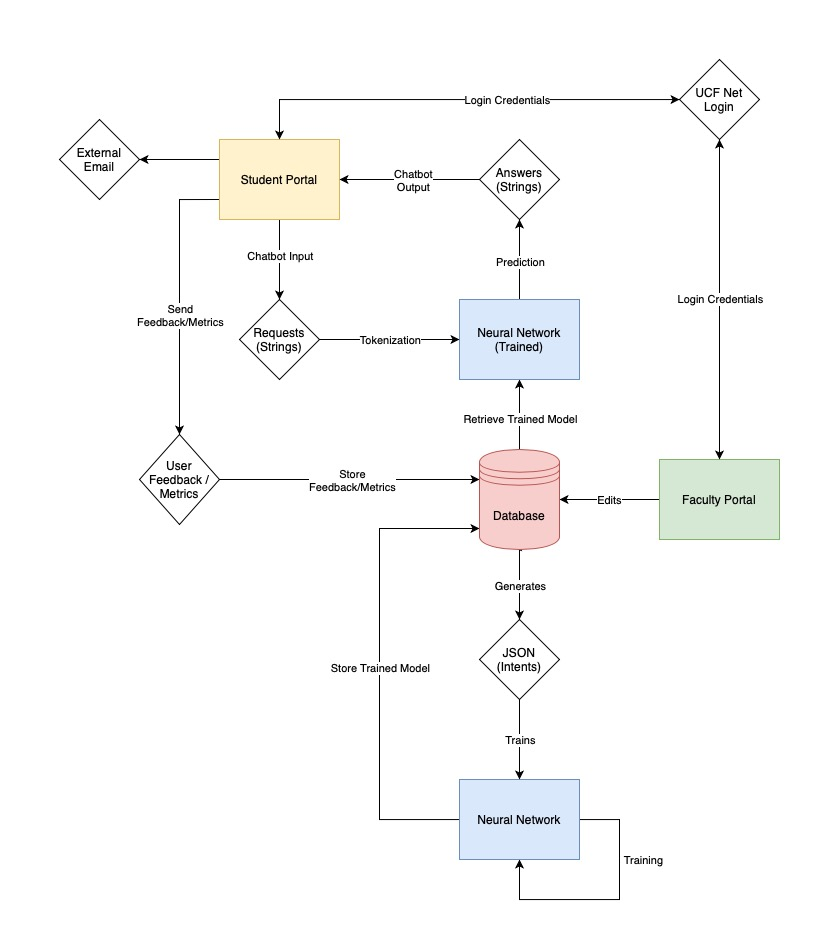
\includegraphics[width=1\linewidth]{images/system-design.jpg}
    \caption{Chatbot System Design}
\end{figure}

\pagebreak

\begin{figure}[h]
    \centering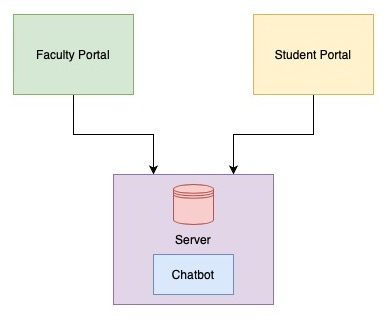
\includegraphics[width=0.5\linewidth]{images/high-level-design.jpg}
    \caption{Chatbot High-Level Design}
\end{figure}

Further, sections (???) through (???) provide in more detail the system design for each component.

\subsection{AI System}

The chatbot system is composed of two main sub-components: (a) an AI-powered neural network for natural language understanding (NLU) and (b) a retrieval-based system for presenting accurate and relevant information to the use. Further, this section also outlines how data will be represented to and from the neural network in the form of a JSON based API file.

\subsubsection{Chatbot Data}

Before outlining the detailed design of the chatbot system, it is important to describe in detail how the data will be represented. The data for the chatbot will be represented using four important artifacts, outlined in Table (???).

\begin{center}
\begin{table}[h]
    \centering
    \begin{tabular}{ L{3cm} L{9cm} }
        \toprule
        \textbf{Artifact} & \textbf{Description}
        \tabularnewline
        \midrule
        Trained Neural Network File & This file will contain all the necessary weight values as determined by the neural network’s training stage. Every time a question is edited, the neural network will be retrained, resulting in the latest version of this file. This file will then be used to get the intents from the input string in the chatbot system.
        \tabularnewline
        \midrule 
        Intents File & This file will contain an array of intents, each of which have a corresponding tag and array of patterns. This file is read by the chatbot back-end to allow the neural network to recognize intents. Figure (???) show a casual representation of this file.
        \tabularnewline
        \midrule
        Knowledge Base & The knowledge base will be the part of the database concerned with storing and cataloguing all categories, questions, and responses. Once the enroll network detects intents, these are mapped to entities that are searched in the knowledge base to look for appropriate responses. Section (???) dives deeper into the structure of this sub-component.
        \tabularnewline
        \bottomrule
    \end{tabular}
    \caption{Artifacts in the AI system.}
\end{table}
\end{center}


\begin{figure}[h!]
    \centering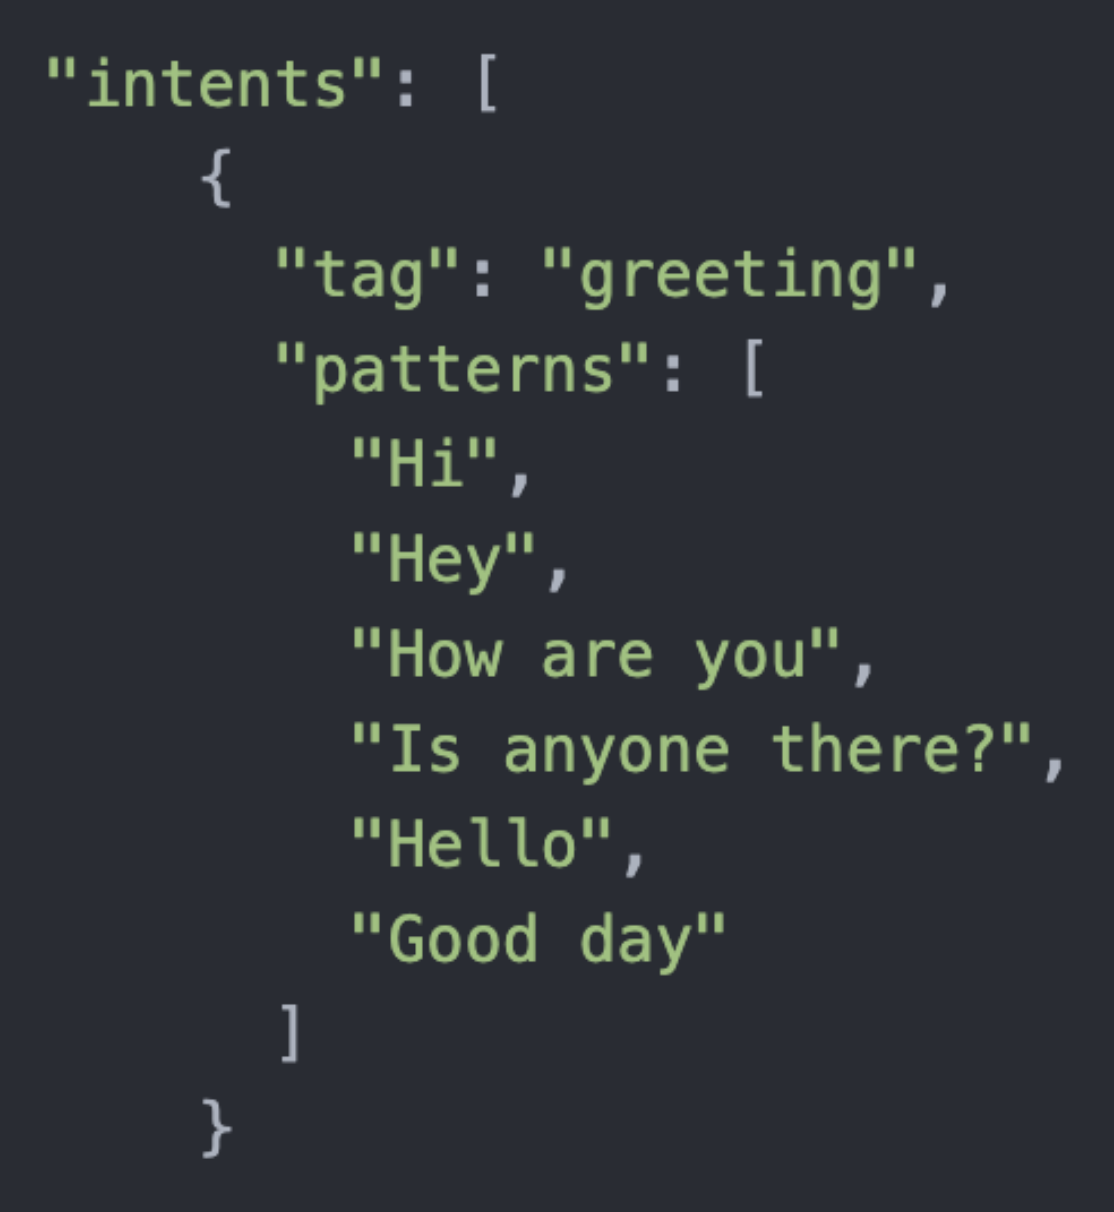
\includegraphics[width=0.5\linewidth]{images/json.png}
    \caption{An example of an intent formatted in a JSON file.}
\end{figure}

\subsubsection{Neural Network}

At the heart of the chatbot system is an AI-powered neural network. This model will handle the process of natural language understanding (NLU), outlined in section (???). Here, the network will be able to understand user input in the form of intents. This is done by feeding the input string into the neural network, which will then output a probability value for each intent found in the database. Figure (???) shows a visual representation of the model’s architecture. Here, p = the number of patterns of bags in the bag-of-words representation, and t = the number of tags.

\begin{figure}[h!]
    \centering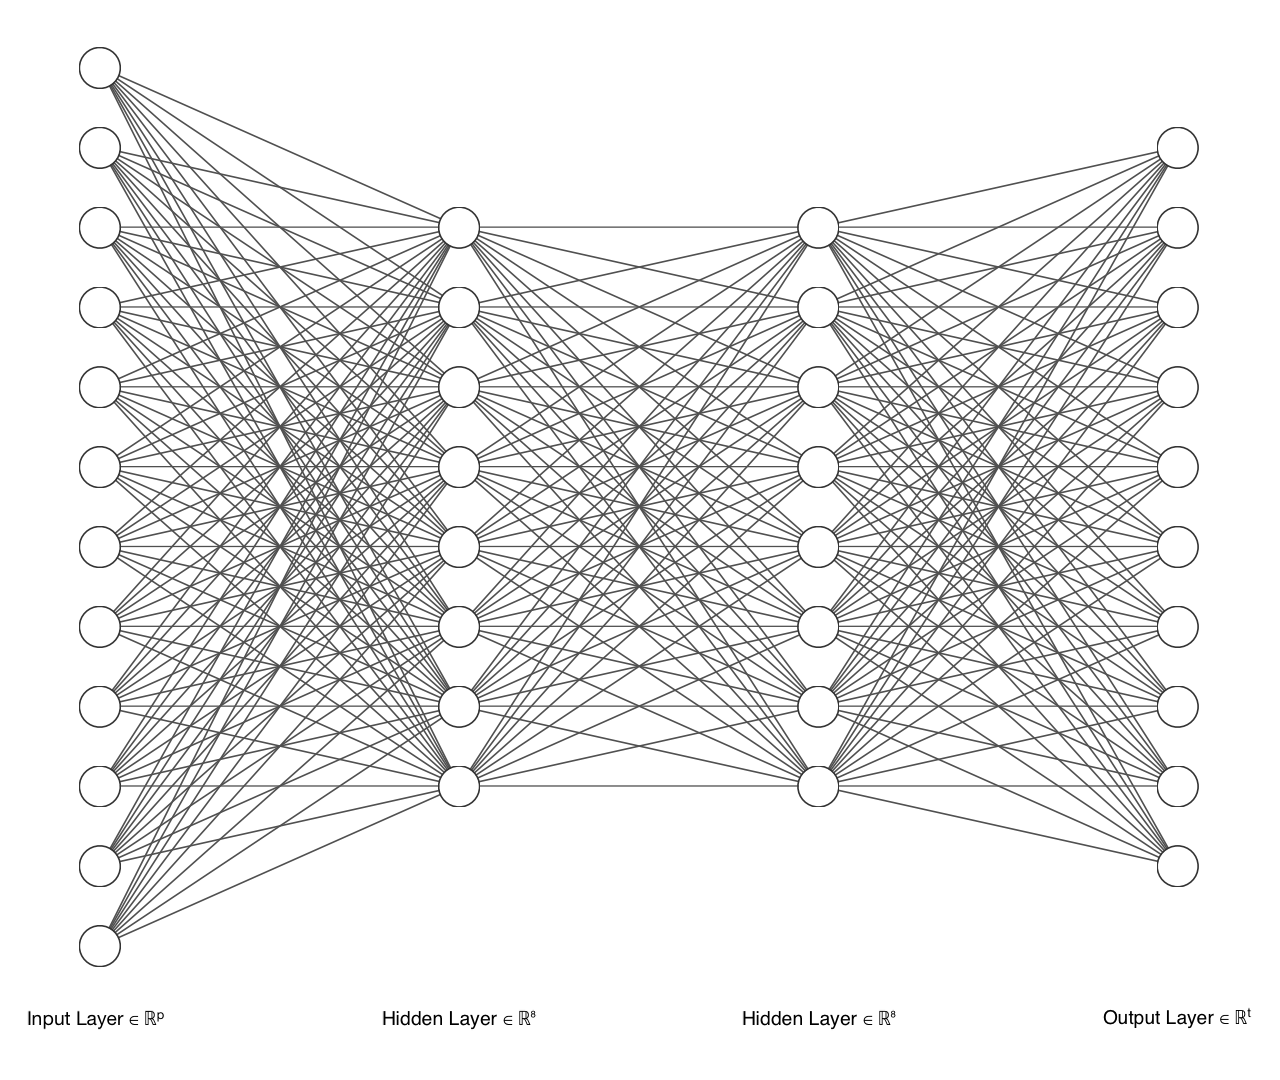
\includegraphics[width=0.875\linewidth]{images/nn-architecture.png}
    \caption{The architecture of the system's neural network.}
\end{figure}

\subsubsection{Retrieval-Based System}

What follows the neural network is the sub-component that powers the greater retrieval-based chatbot system. Here, the intents understood by the neural network are mapped into entities, which reside in the knowledge base system. The system will then search for these entities in the knowledge base, looking for a response to the question asked by the user. The following steps outline this process:

\begin{enumerate}
    \item When a user types a question, the string input and the current context is received from the student system via an API call.
    \item Once this string is received, an API call will be made to the database system to get the latest trained neural network model and intents file.
    \item When all the files are in place, the input string is then tokenized using a bag-of-words approach. This filters out any stop words to continue with the NLU process.
    \item Once the input tokens are ready, they are fed into the trained neural network.
    \item The neural network will then output a series of probability values, one for each intent found in the intents file.
    \item The intents found will then be chosen by using a probability distribution that will be determined during the testing phase.
    \item These intents will then be mapped to entities found in the knowledge base. These entities will be used by the knowledge base system to find the appropriate response to the original question.
    \item Further, starting from the highest entity level, a context hierarchy will be established.
    \item The retrieval-based system will finally send the response to the question and the current context back to the student system via an API call.
\end{enumerate}

Further, Figure (???) shows a visual representation of this process. Here, we can see how the chatbot system receives input, asks for clarification when needed, and responds appropriately.

\begin{center}\emph{[ FIGURE COMING SOON ]}\end{center}

\subsection{Student System}

The chatbot should feel intuitive and provide an easy method of communication for the user, making use of things like buttons for questions with limited answer choices and the ability to ask Knugget to clarify something. The API calls should allow for the most efficient and effective delivery of information to the user. Knugget’s (the chatbot’s) personality should make it fun for the user, but not distract from the purpose of the app.

The following section contains in-detail a component-wide design of the student system.

\subsubsection{Front-End}

\textbf{User Input}

The user will submit input either by typing or speaking words into the chat, like a text message, or by clicking buttons. It is important that the user be guided into submitting input in a way that is efficient in receiving the appropriate answers. One way that this can be done is by presenting the user with buttons when applicable and convenient. For instance, when the chatbot is trying to determine what it is being asked by the user, it is keeping track of entities.

When all entities are matched, then the chatbot can determine if there is an answer appropriate for the question or comment:

\begin{itemize}
    \item If there is more than one entity that has not been matched and more than one item is returned from the knowledge base, then the chatbot will continue to ask questions.
    \item If there is more than one item returned and there is only one entity match missing, then buttons will be generated as an option for the user.
    \item If there is only one item returned, under any circumstances, then that is the final answer that the chatbot will be able to give without matching different entities afterward.
\end{itemize}

\textbf{User Interface/Experience}

The user output can be designed in such a way that it is clear if the messages were written by the chatbot or the user, for the ability to go back and review what has been said. One way to do this is by spacing the messages so that the chatbot’s messages appear on the right and the user’s messages appear on the left. Another way is by putting an icon next to each message which can be easily associated with the correct party. For example: Knugget (the chatbot) can be represented by a pony icon. The icon is the best way to represent who said what, but things like indentation and color may also be used. Further, Figure (???) shows a visualization of these UI components in action.

\begin{center}\emph{[ FIGURE COMING SOON ]}\end{center}

\subsubsection{Back-End}

\textbf{API Endpoints}

In the back-end for the student system, there will be two major API endpoints:

\begin{enumerate}
    \item Identify (POST Request)
    \begin{itemize}
        \item One API endpoint is an “identify” endpoint. This endpoint will be a post request. This means that this will be used when the chatbot will need to parse what has been said before going to the knowledge base and answering the user’s question on the front-end.
        \item The front-end will call this endpoint when the user types a question or response into the chat box. This chat message will go to the AI system to be parsed, then to the neural network to be understood, and then to the knowledge base to determine the correct, next action to take.
        \item After this, the front-end will display that action and allow the user to submit more input.
        \item The output upon successful completion will be some string of text, the new context for the client, and a record of the completion case that it is on.
    \end{itemize}
    \item Known (POST Request)
    \begin{itemize}
        \item The “known” endpoint is very similar to the “identify” endpoint, except that the input is not parsed in the AI system, because it is already known what the input means. This endpoint will be a post request.
        \item This endpoint will be used when the user is presented with buttons to click and the user decides to click one of those buttons instead of typing a chat message.
        \item For example: if the user is given a “yes” and a “no” button, then it will already be known what either of those responses means, should the user click one of them. However, if the user typed “affirmative”, “nay”, “that sounds good to me- please do that”, etc., then the input would have to be parsed to determine what that means. 
        \item The output upon successful completion will be some string of text, the new context for the client and a record of the completion case that it is on.
    \end{itemize}
\end{enumerate}

\textbf{Email}

The main purpose of this chatbot is to decrease the amount of email Dr. Mark Heinrich and other advisors receive. However, there are times when sending an email is unavoidable. In these times, it is best to send as few emails as possible. This can be accomplished by gathering all the required information beforehand. Because we were given what information Dr. Heinrich would need from a student given a certain circumstance, the chatbot can ask the student to provide all of the information to it. If and when all the information is provided to the chatbot, an email can be sent to the professor. The email will include all of the required information and the student’s Knights email address so that the advisor can reply directly to the student, if necessary. The ideal outcome in a situation where an email would have to be sent would be for the chatbot to send an email to the advisor and the advisor would be able to do what the student needs them to do without the advisor asking for additional information. This saves the advisor’s time, but also the student’s time.

\subsection{Faculty System}

One of the main components of our product is a faculty system that gives advisors the right and privilege to add, delete and modify the chatbot instructions, data and interpretations as per their need and requirement. 

Sometimes, they need to add a list of new questions being asked that the chatbot may not recognize or cover, such as “How does COVID-19 affect my class requirement?” This question would have never been asked before the COVID-19 pandemic, hence new circumstances like these may lead to the possibility of new questions that are unknown to the chatbot.

Therefore, it is important to have a system from where the advisors can add this type of questions or somehow train the existing model that we create, with an easier and user-friendly approach.

\subsubsection{Back-End}

\textbf{API Endpoints}

Much like with the student system, the faculty system also contains many different API endpoints as part of its back-end component. These are outlined below:

\begin{enumerate}
    \item get-entity-sets (GET request)
    \begin{itemize}
        \item Used to retrieve the list of entities and entity sets in the knowledge base. This includes the name and ID of each entity-set along with the names and IDs of all entities belonging to said entity-sets, all of which should be formatted as JSON.
        \item The request is then passed to the database manager which it retrieves the information from the knowledge base. This information is then returned to the front-end.
        \item If, for some reason, the entity-sets and their entities could not be retrieved, a failure message will be returned to the front-end to be displayed to the user.
    \end{itemize}
    \item get-entity (POST request)
    \begin{itemize}
        \item Used to retrieve the information for a specific entity. This information includes the entity’s ID, name, and associated patterns, all of which should be formatted as JSON.
        \item As input, the function takes in the IDs of both the entity to be retrieved and the entity set it belongs to formatted as JSON. It then sends those IDs to the database manager to retrieve the requested information.
        \item Upon successful retrieval, a success message is returned to the front-end along with the information for the requested entity.
        \item If, for some reason, the entity’s information could not be retrieved, a failure message will be returned to the front-end to be displayed to the user.
    \end{itemize}
    \item create-entity-set (POST request)
    \begin{itemize}
        \item Used to add a new entity-set to the knowledge base. As input, the function takes in the name of the new entity-set. The name is then sent to the database manager to be added to the knowledge base.
        \item Upon successfully adding the name to the knowledge base, a success message is returned to the front-end along with the name and id of the newly added entity-set.
        \item If, for some reason, the entity-set could not be added to the knowledge base (such as in the case of there already existing an entity set with the same name) a failure message will be returned to the front-end to be displayed to the user.
    \end{itemize}
    \item create-entity (POST request)
    \begin{itemize}
        \item Used to add a new entity to an entity-set in the knowledge base. As input, the function takes in the name of the new entity, the ID of the entity-set it belongs to, and the patterns used to recognize the entity, all of which should be formatted as JSON.
        \item This information is then sent to the database manager to be added to the knowledge base.
        \item Upon successfully adding the entity to the knowledge base, the function then sends a message to the AI system to retrain the model. Once the model has been successfully trained on the knowledge base including the new entity, a success message is sent to the front-end along with the name, ID, and training statistics for the new entity. 
        \item If, for some reason, the entity could not be added to the knowledge base or if there was an issue with the training, a failure message is sent to the front-end to be displayed to the user.
    \end{itemize}
    \item update-entity-set (PUT request)
    \begin{itemize}
        \item Used to update the name of an entity-set in the knowledge base. As input, the function takes in the id and name of the entity-set to be updated and the new name it should have, all of which should be formatted as JSON.
        \item This information is then sent to the database manager to update the knowledge base. Upon successfully updating the entity-set, a success message is returned to the front-end.
        \item If, for some reason, the entity-set could not be updated, a failure message will be returned to the front-end and displayed to the user and the original name should be preserved.
    \end{itemize}
    \item update-entity (PUT request)
    \begin{itemize}
        \item Used to update information regarding a specific entity currently in the knowledge base. As input, the function takes in the ID, name, and existing patterns for the entity, along with the potential new name and potential new patterns, all of which should be formatted as JSON.
        \item This information is then sent to the database manager to update the knowledge base with the new name and/or patterns.
        \item If the new name is different from the existing name, all questions which used this name will also be updated to reflect the name change.
        \item If the patterns were changed, the function will send a message to the AI system to re-train the model based on the new patterns.
        \item Upon successfully updating the knowledge base, a success message will be returned to the front-end, to be displayed to the user. If the model was re-trained, the training statistics are returned with the success message.
        \item If, for some reason, the entity could not be updated or if there was an issue with the training, a failure message is sent to the front-end, to be displayed to the user.
    \end{itemize}
    \item delete-entity-set (DELETE request, Admin only)
    \begin{itemize}
        \item Used to remove an entity-set, all associated entities, and all associated questions from the knowledge base. The function takes in the name and id of the entity-set to be deleted formatted as JSON.
        \item It then passes that information to the database manager to find all entities in the entity set and all questions which use those entities.
        \item The IDs of those questions are then sent to the database manager to be deleted. The IDs of the associated entities are then sent to the database manager to be deleted. Finally, the ID of the entity-set is sent back to the database manager to be deleted.
        \item Upon successful deletion of all items, a success message is returned to the front-end and displayed to the user.
        \item If, for some reason, anything could not be deleted in this process, a failure message will be returned to the front-end, to be displayed to the user, and the knowledge base should preserve its state from before the function was called.
        \item Due to the highly destructive nature of this command, it will only be accessible to users authorized as administrators for KnugBot.
    \end{itemize}
    \item delete-entity (DELETE request, Admin only)
    \begin{itemize}
        \item Used to remove a specific entity and all associated questions from the knowledge base. The function takes in the name and id of the entity to be deleted formatted as JSON.
        \item This information is then sent to the database manager to delete all questions which use this entity from the knowledge base before deleting the entity itself.
        \item Upon successful deletion, a success message is returned to the front-end and displayed to the user.
        \item If, for some reason, the entity or its associated questions could not be deleted, a failure message is returned to the front-end and displayed to the user and the knowledge base should preserve its state from before the function was called.
        \item Due to the highly destructive nature of this command, it will only be accessible to users authorized as administrators for KnugBot.
    \end{itemize}
    \item get-questions (GET request)
    \begin{itemize}
        \item Used to retrieve the list of all current questions in the knowledge base. This includes the question id and the question nickname formatted in JSON.
        \item The request is passed to the database manager which retrieves this information from the knowledge base. This information is then returned to the front-end.
        \item If, for some reason, the questions could not be retrieved, a failure message is returned to the front-end to be displayed to the user.
    \end{itemize}
    \item get-question (POST request)
    \begin{itemize}
        \item Used to retrieve the information for a specific question from the knowledge base. This information includes the ID, nickname, associated entities and which entity-sets they belong to, and the possible responses to that question, all of which should be formatted as JSON.
        \item As input, the function takes in the ID of the question formatted as JSON. It then sends that ID to the database manager to retrieve the necessary information.
        \item Upon successful retrieval, a success message is returned to the front-end along with the requested information.
        \item If, for some reason, the question could not be retrieved, a failure message is returned to the front-end to be displayed to the user.
    \end{itemize}
    \item create-question (POST request)
    \begin{itemize}
        \item Used to create a new question in the knowledge base. As input, the function takes the entities used to make up this question and the possible responses, all of which should be formatted as JSON.
        \item This information is then sent to the database\_manager to be added to the knowledge base.
        \item Upon successfully adding the question to the knowledge base, a success message is returned to the front-end, to be displayed to the user, along with the ID and name of the new question.
        \item If, for some reason, the question could not be added to the knowledge base, a failure message is returned to the front-end to be displayed to the user.
    \end{itemize}
    \item update-question (PUT request)
    \begin{itemize}
        \item Used to update the list of potential responses for a specific question. As input, the function takes the ID of the question to be updated, the old list of potential responses, the old list of identifying entities, the new list of potential responses, and the new list of identifying entities, all of which should be formatted as JSON.
        \item This information is then passed to the database manager to update the knowledge base.
        \item Upon successfully updating the question in the knowledge base, a success message is returned to the front-end to be displayed to the user.
        \item If, for some reason, the question could not be updated, a failure message is returned to the front-end, to be displayed to the user, and the original question information should be preserved.
    \end{itemize}
    \item delete-question (DELETE request)
    \begin{itemize}
        \item Used to remove a specific question from the knowledge base. As input the function takes in the ID of the question to be removed.
        \item This is then sent to the database manager to delete the question from the knowledge base.
        \item Upon successful deletion of the question from the knowledge base, a success message is returned to the front-end and displayed to the user.
        \item If, for some reason, the question could not be deleted, a failure message is sent to the front-end and displayed to the user.
    \end{itemize}
    \item get-contacts (GET request)
    \begin{itemize}
        \item Used to get the list of contacts from the knowledge base. This includes the contact ID, contact name, contact title, and contact email all formatted as JSON.
        \item The request is passed to the database manager which retrieves this information from the knowledge base. This information is then returned to the front-end.
        \item If, for some reason, the questions could not be retrieved, a failure message is returned to the front-end.
    \end{itemize}
    \item create-contact (POST request):
    \begin{itemize}
        \item Used to add a new contact to the knowledge base. As input, the function takes in the name, title, and email of the new contact, all formatted as JSON.
        This information is then sent to the database manager to be added to the knowledge base.
        \item Upon successfully adding the contact to the knowledge base, a success message is returned to the front-end, to be displayed to the user, along with the ID, name, title, and email of the new contact. 
        \item If, for some reason, the contact could not be added to the knowledge base, a failure message is returned to the front-end, to be displayed to the user.
    \end{itemize}
    \item update-contact (PUT request)
    \begin{itemize}
        \item Used to update an existing contact in the knowledge base. As input, the function takes in the ID, old name, old title, old email, new name, new title, and new email for the contact to be updated, all of which should be formatted as JSON.
        \item This information is then passed to the database\_manager to be updated in the knowledge base.
        \item Upon successfully updating the contact in the knowledge base, a success message is returned to the front-end to be displayed to the user.
        \item If, for some reason, the contact could not be updated, a failure message is returned to the front-end, to be displayed to the user, and the original contact information should be preserved.
    \end{itemize}
    \item delete-contact (DELETE request)
    \begin{itemize}
        \item Used to delete a contact from the knowledge base. As input, the function takes in the ID of the contact to be deleted formatted as JSON.
        \item This is then passed to the database manager to be deleted from the knowledge base.
        \item Upon successfully deleting the contact from the knowledge base, a success message is returned to the front-end to be displayed to the user.
        \item If, for some reason, the contact could not be deleted, a failure message is sent to the front-end and displayed to the user.
        \item While this function will be provided, it is primarily intended for cases where a particular contact is genuinely no longer needed.
        \item If a certain position is being filled by a new person, it would be advised that the contact associated with that position be updated rather than deleting the contact and adding a new one.
    \end{itemize}
\end{enumerate}

























































\pagebreak



% Section: Testing (DONE)
\section{Testing}

% Needs citation.
A chatbot’s function can be tested through application of user stories or through other forms of live testing. It may be beneficial to, even before any development takes place in Senior Design II, design a flowchart based upon expected user interactions. Additionally, a prototype can be useful in these early stages. Prototyping tools such as Botsociety and Sketch + Marvel can be utilized to solidify plans for how the chatbot will function. It is also recommended that content required for building the chatbot, as previously described, be compiled and compared in a document like an Excel spreadsheet. Once completed, this sheet can be used as instruction for developers, so that they can best implement the design. Once a chatbot or a prototype is able to receive and respond to user input, the best way to ensure proper function is through rigorous user testing [3].
 
In user testing, it is imperative that documentation be thorough. Every time that the interface’s response diverges from what is expected, the response should be recorded so that discovery of what is wrong can be as efficient as possible. When testing, it is important to put oneself into the “shoes” of the user. What technological abilities does that user have? What could their intentions be for interacting with the software? Is it possible that a user would intentionally try to break the software or cause it to do something that is not supposed to do? These questions should be considered and plans for combating negative outcomes should be formed.

\subsection{AI System}

In terms of testing, the AI component of the product will have to be thoroughly vetted to ensure it works as intended. The success of the entire product depends in large part to the success of the main AI system.

To ensure this system does a quality job, three main testing methods will be used: (a) neural network training loss, (b) natural language understanding (NLU) accuracy, and (c) retrieval accuracy.

\subsubsection{Neural Network Training Loss}

The first performance metric for this component will be the training loss. During the training phase, the binary cross-entropy loss metric will be used and minimized with an Adam optimizer. Here, the goal in testing will be to minimize this loss by changing the training parameters, including the (a) learning rate, (b) weight decay, etc. The neural network architecture itself may also be edited to further improve this score by attempting to find the optimal configuration of number of layers, hidden units, activation functions, and using state-of-the-art, deep learning techniques.

\subsubsection{Natural Language Understanding (NLU) Accuracy}

Another important part of the AI component is having the neural network accurately understand user intent. To measure this, a custom dataset will be generated specifically for testing. Here, the dataset will be composed of sample input strings and ground-truth intent keywords as labels. Table (???) shows an example of this dataset.

\begin{center}
\begin{table}[h]
    \centering
    \begin{tabular}{ L{6cm} L{6cm} }
        \toprule
        \textbf{Input String} & \textbf{Intents}
        \tabularnewline
        \midrule
        “When is the deadline to take the foundation exam?” & “deadline”, “take”, “foundation exam”
        \tabularnewline
        \midrule 
        “How do I sign up for the accelerated BS-to-MS program?" & “how”, “sign up”, “bs-to-ms”
        \tabularnewline
        \midrule
        “Can I get an override into a graduate course?” & “override”, “graduate”, “course”
        \tabularnewline
        \bottomrule
    \end{tabular}
    \caption{Sample dataset of input strings and intents.}
\end{table}
\end{center}

Once this dataset is constructed based on the questions and responses in the knowledge base, it will be used to test the neural network and provide an accuracy score. The higher this score, the more reliable the NLU system.

\subsubsection{Retrieval Accuracy}

Finally, to measure the accuracy of the retrieval sub-component, another custom dataset will be built to ensure it works at the highest quality possible. Here, a list of sample interactions with the chatbot will be provided along with a list of response strings as the ground-truth label. Table (???) shows an example of this dataset, which will give an insight into how well the system is actually responding to relevant questions.

\begin{center}
\begin{table}[h]
    \centering
    \begin{tabular}{ L{6cm} L{6cm} }
        \toprule
        \textbf{Interactions List} & \textbf{Response List}
        \tabularnewline
        \midrule
        “When is the deadline to take the foundation exam?” & “The deadline to take the foundation exam is \_\_\_.”
        \tabularnewline
        \midrule 
        “BS-to-MS program.”, “How do I sign up?” & “What would you like to know about the accelerated BS-to-MS program?”, “To sign up, perform the following steps: \_\_\_.”
        \tabularnewline
        \bottomrule
    \end{tabular}
    \caption{Sample dataset of target interactions and responses.}
\end{table}
\end{center}

This custom dataset will be developed based on the real questions present in the system’s knowledge base. This will allow the team to ensure the component works well with a quantifiable metric.

\pagebreak








\section{Other Proposed Solutions}

In the process of designing a product, original design choices will be changed and modified in order to make way for newer, better designs. There will often be mock-ups, diagrams, research, etc., that do not fit with the current scope of the project, but that does not mean that the effort was in vain. When this happens, it can be beneficial to the end product for the team to understand why one direction was chosen and another was not. When the team decided to go another way, it was important to us that we understood and documented why. Taking time to critique the reasons that something was not ideal and to explain why the new way was better helped to solidify our plans and to focus our vision. Additionally, we were told before writing this document that we should present the information in a way that would help another team to understand and execute our design. In that circumstance, this section would contain indispensable knowledge that would save the team time and energy that could be spent more efficiently elsewhere.

\subsection{AI System}

\subsubsection{Choosing the Right Chatbot Technique}

Using natural language processing techniques can be very beneficial in the development of our chatbot. Therefore, as part of our research, we explored how such a system could work with or without this approach.

Initially, we explored the possibility of using a purely rule-based chatbot. This approach was a bit simpler compared to the NLP approach in regard to the advisor front-end experience. In this one we thought we could add a new question and a response to it without having to train the chatbot model or collect any past data. The front-end design would have been much like a form that takes in inputs from the advisor who has the privilege to add, delete, and update information in the database using the proposed front-end system.

For example, consider an advisor wanting to add new questions related to the COVID-19 pandemic. We could have used a tags list which had all the questions already known to the chatbot that related to coronavirus and the advisor could have then added these new questions and assigned the specific tags to those questions. Similar to the questions, another idea was to implement the same tag system with the responses as well. If more than one question had the same answer it would have been very efficient to just type the answer once and then reuse the tag for every time the response was the same.

However, upon further research, we decided to use a fully NLP-based chatbot system instead. This approach requires the model to be trained frequently, as changes are made to the system. So in our case, if we need to add a new question, there has to be some sort of training involved. To train this model we need some training data that can be used to train the chatbot. In this case, we will be employing the use of a dedicated knowledge base system that will contain all the necessary information for the AI system to learn. This data can be used as an input from the advisor in their front-end system with entities and related responses to those entities/data. It is possible to make an efficient front-end system that communicates with the back-end database using APIs. In the front-end they will be able to enter a collection of data that relates to training the chatbot for adding new questions.

Each approach is very unique and different in its own way, but we believe we made the right choice moving forward.


\subsubsection{Choosing the Right Chatbot Development Platform}

At the beginning of our research endeavor, we explored the possibility of using dedicated, out-of-the-box chatbot systems to simplify our development process. However, cost for this project was a concern, so we ultimately decided against it. Nonetheless, below is a summary of our findings for each major development platform:

\textbf{Amazon Lex}

Released in 2017, Amazon Lex is Amazon's response to the chatbot revolution in the last decade. The following are some highlights from our research:

\begin{itemize}
    \item It is a service for building "conversational interfaces" into applications, making use of both voice and text.
    \item Currently powering Amazon's Alexa virtual assistant, it uses deep learning for automatic speech recognition (ASR) and natural language understanding (NLU), bringing these cutting-edge technologies to the hands of developers.
    \item Fully-integrated with Amazon Web Services (AWS), this system provides an end-to-end solution with high-quality interactions and easy deployment.
    \item In terms of pricing, it follows a "pay for what you use" system, charging \$0.004 per voice request, and \$0.00075 per text request. For example, they state that 500 speech and 500 text requests would cost a total of \$2.38 per month.
\end{itemize}

Overall, this originally seemed like a good contender, but our ultimate decision was to pursue a different avenue.

\textbf{Azure Bot Service}

Microsoft's Azure Bot Service is marketed as a way to develop intelligent enterprise bots while maintaining control of the data. Further points from our research include:

\begin{itemize}
    \item It allows developers to build essentially any kind of chatbot, from simple FAQs to multi-faceted virtual assistants.
    \item Further, it makes use of Bot Framework, an open-source SDK with tools for end-to-end bot development.
    \item As for pricing, they offer competitive prices, having a free tier of unlimited messages in standard channels and 10,000 messages per month in premium channels. However, it gets rather confusing when they state that other Microsoft services may be needed, such as an optional provision of Application Insights.
\end{itemize}

The pricing was very competitive, as it provided a generous free option, but it was also scrapped after more research was conducted.

\textbf{IBM Watson Assistant}

According to IBM's official website, Watson Assistant is the "industry leading conversational AI technology powering chatbots." Our research produced the following key points:

\begin{itemize}
    \item Like the other platforms surveyed in this document, it focuses on having a powerful AI system powering it, ensuring efficiency, power, and ease of deployment.
    \item Watson Assistant also provides many powerful integrations, although their use to our project may be up for debate.
    \item In terms of pricing, it starts to get much more complicated. While it has a similar system to Microsoft's Azure Bot Service, including 10,000 messages a month in its free tier, it also imposes a limit to the number of users, capping it at 1,000 per month. Further, if the free tier is not enough, the unforgiving price of \$120/month for the Plus tier is what follows, making it a very difficult platform to recommend.
\end{itemize}

While this might be the best platform currently available on the market, its steep price points made this platform far from our financial reach.

\textbf{Google Dialogflow}

Google markets their Dialogflow platform as an "advanced development suite for creating conversational AI applications, including chatbots, voicebots, and IVR bots." The following key points were also gathered from our research:

\begin{itemize}
    \item It gives very similar features to the other platforms described in this document, but it seems to excel in having very thorough documentation. Further, from all the systems, this seems to be the most straightforward in terms of development.
    \item However, its pricing system is not at all friendly. Charging \$0.002 per text request and \$0.0065 per 15 seconds of audio requests, it is evident that it may also be beyond our reach, as these numbers are sure to quickly begin adding up. 
    \item Further, they charge extra for sentiment analysis and the provision of audio outputs, charging \$4 per one million characters.
\end{itemize}

Like the other platforms, Google Dialogflow's great features and excellent documentation were not enough to justify its steep pricing.

\textbf{Wit.ai}

Wit.ai seemed to be a great contender, especially because it is a free service. Further, other research points included:

\begin{itemize}
    \item It seems to have similar features to the other premium services outlined, including reminders, contextual information, etc.
    \item By far, Wit.ai's greatest draw is its pricing. However, it is important to know that no service is truly free. It is very well-known that whenever a service is free, the user is the product. These suspicions are further exacerbated when reading that Facebook acquired the system not long ago. Therefore, privacy is a genuine concern, especially since we are working with confidential information, some of which is data that is FERPA-regulated.
\end{itemize}

Therefore, this idea was not pursued, as we must keep the security and privacy of our users at the forefront.

\textbf{BotPress}

With further research, another interesting platform was found. BotPress, seen by many as the WordPress for chatbots, is marketed as the "leading open-source conversational AI platform for enterprise automation." The research conducted also provided the following points:

\begin{itemize}
    \item With the flexibility of open-source comes an excellent free tier.
    \item They also give an emphasis on privacy, which sets it above Wit.ai on this front. Further, used by organizations such as Duke, Verizon, and BBVA, they make their money by presenting a paid Enterprise version.
    \item They also provide a thorough SDK.
    \item However, the fact that it is open source makes it much more scalable and long-lasting, as even if the organization goes out of business, we would still have access to our code.
\end{itemize}

Finally, like with the other platforms, we decided to no longer pursue this route.

\subsection{Faculty System}

The faculty system was another major component of our product that changed a lot as we designed it. The current design can be found on section (???), and below we outline various ideas we were working with at the beginning our design process.

\subsubsection{Front-End}

The initial prototype design we had was primarily based on the assumption of using a strictly rule-based chatbot model in terms of how it expects adding new questions to function. However, some of these items did make their way to the final design. Below are some examples of how this looked in its infancy.

\textbf{Overview}

The basic requirements of the front-end system included: a login authentication system that would only allow the advisors and people with authorized credentials to make an account and log in. Furthermore, we also had decided to use the UCF login credentials and use their APIs for authentication. This was then confirmed after meeting with the UCF IT team.

We also needed:

\begin{itemize}
    \item A way to input new data.
    \item A tag drop-down.
    \item A search bar to look up relevant tags and questions.
    \item A button for generating the statistics related to the most popular questions that have been asked by users/students.
    \item A way to delete data or update it when needed.
    \item An input element for responses and a checkbox for the tag names it can be associated with that are given based on the priority and correlation.
\end{itemize}

In addition, as shown in the design diagram, the advisor would be able set limitations to the input and have them do only specific tasks like generate template, send emails, etc.

Another functionality that was included in the original front-end design was the infrastructure to allow or open up the opportunity for other departments to have a chatbot for their specific department. With that infrastructure in place, it would be easy for future teams to launch a design in which each departments’ advisor can add/delete/edit questions and responses for the chatbot ‘only’ for their specific department. This would really lay a concrete groundwork for the future projects to expand our idea and help our advisors and the student body efficiently. This is an idea that we fully embraced in the final design.

\textbf{Landing Page}

The initial landing page was be the primary location where advisors could look through, add, delete, and edit questions and their responses. This design focused on ensuring ease of use and ease of understanding for the advisors while minimizing the amount of time spent searching for specific features/functions.

To avoid bombarding users with more information than they may need in a given session, advisor contact information and statistical information about the chatbot were located in their own tabs. When selecting another tab, the \emph{Categories} column remains fixed as a means of providing some manner of filtering results. However, while in the \emph{Advisor Directory} tab, the \emph{Questions} column would become the \emph{Directory} column to provide a list of existing contacts within the system, whether they be individual advisors or general departments.

\begin{figure}[h]
    \centering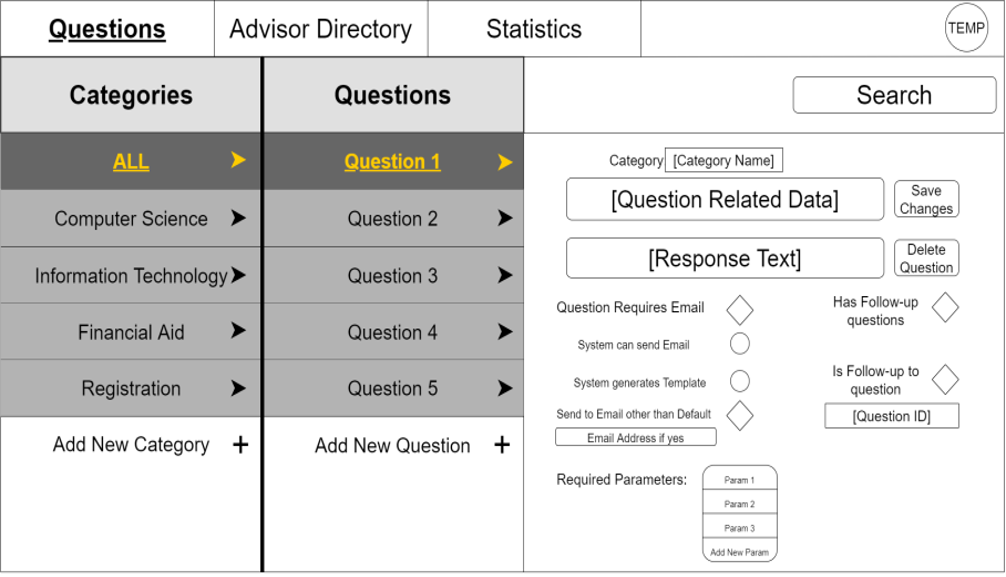
\includegraphics[width=1\linewidth]{images/original-landing-page.png}
    \caption{The original landing page.}
\end{figure}

\textbf{Categories}

This section of the landing page is used to filter questions by specific Category. Separating questions by Category serves several purposes:

\begin{itemize}
    \item It allows advisors to find a question they may be looking for more quickly by letting them filter out unrelated questions.
    \item It allows the system to define a default contact for each category, thereby streamlining the process of filling in responses to new questions.
    \item It allows for the expansion of the system beyond the CS and IT majors, as should another department wish to make use of the application for their advising office as well, all they would have to do is add a new Category for that major and begin adding new questions and responses.
\end{itemize}

Further, an example of the original design for the \emph{Categories} panel can be viewed in Figure (???).

\begin{figure}[h]
    \centering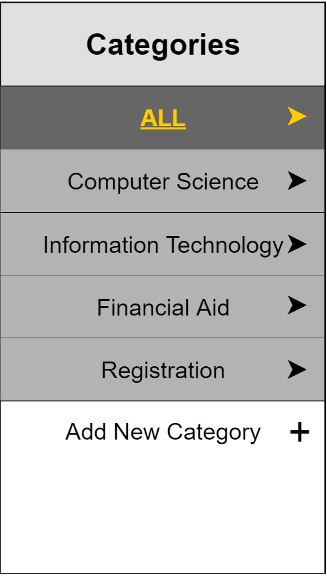
\includegraphics[width=0.5\linewidth]{images/original-categories-panel.png}
    \caption{The original categories panel.}
\end{figure}

\subsubsection{Back-End}

\textbf{Form Handling}

As part of the back-end, we need a way for the advisors to constantly keep and update on the forms that students may get in response from the chatbot. To handle this specific task,  there are two ways that we were considering going about solving it:

\begin{enumerate}
    \item Advisors could upload new forms or update new forms with an upload section in the front-end which would then store the relevant form with the tag associated to it, in the database.
    \item The chatbot never actually responds the actual/physical PDF of the form. Instead it just directs them with a link to the form where it could be found on the UCF website.
\end{enumerate}

Considering these two solutions, the first one made it easier for the user to locate a specific form, and the advisor to add a new form, as there can be cases where a particular form is nowhere to be found on the UCF website. This required further research, including about how to write these APIs and security issues that could arise with the functionality being made available to students as well as the advisors. An administrator had to have control of these things and overlook each and every action depending on the sensitivity of the subject matter. These are all things that were addressed in the final design.

\textbf{Question Handling}

All questions recognized by the system would appear in the \emph{Questions} column. An example of this preliminary design can be found on Figure (???). Choosing a specific category would allow advisors to narrow down the breadth of questions they’re looking through, with a search bar in the upper right-hand corner to help narrow down existing questions even further. That search bar would only ever display results from the current category, so if an advisor is searching for a specific question to update its response and they can’t find it, it may help to check a different category, or perhaps even click the \emph{All} category to see all existing questions. Once a question had been selected, the right pane of the application would be populated with the question’s information including:

\begin{itemize}
    \item If the final product followed a rule-based approach, the text of the question itself.
    \item If the final product followed an NLP approach, some representation of the intents and entities used to make recognize the question.
    \item The response text to be output should the chatbot recognize this question from a user.
    \item The category this question belonged to. If this is initial question creation, rather than question editing, the question would not be submitted as one the chatbot can recognize unless it has a category. 
    \item Whether or not the question had any potential follow-up questions. This would let the system know it should be ready to recognize related questions.
    \item Whether or not the question is itself a follow-up question to some other question or set of questions. If this box was checked, the advisor entering the question would have to identify which questions this one was meant to follow up before the question could start being recognized. 
    \begin{itemize}
        \item It should be noted, the diamond next to the question meatn for our design that you were able to select both at once if you wished. As such, it was possible for a question to both be a follow-up question and to have follow-up questions of its own.
    \end{itemize}
    \item Whether this was a question which required that a student make direct contact with someone, whether it is a UCF CECS advisor or some other department of the university.
    \begin{itemize}
        \item If the diamond stating that a question required some direct communication via email is checked, there were then two possible ways for the chatbot to handle this request. This included:
        \begin{itemize}
            \item The chatbot could send the email on behalf of the student.
            \item The chatbot could generate a template for an email that the student may send at their own time.
        \end{itemize}
        \item These options were marked as circles to denote that they were mutually exclusive. The system was either allowed to send an email on the student’s behalf or it was not. There was no in-between as far as this design is concerned.
    \end{itemize}
    \item Whether, in the event that an email was to be sent, an email would be sent to the default contact listed for the question’s category, or whether it had to go to some other location. The advisor could then enter the alternate email address this response would direct users to.
    \begin{itemize}
        \item This was included as, even in the event every question was always perfectly placed in the correct category, there could still be situations where questions would need to address someone other than the default contact for that category, and so we felt it was wise to allow some provisions for that scenario.
    \end{itemize}
    \item Lastly, should an email be sent, either by the chatbot itself or by a student with a template, if an email was being sent the advisor must specify what parameters, if any, would be sent in the email from the student.
    \begin{itemize}
        \item The first two parameters would always be \emph{Name} and \emph{UCF ID} by default, as those are the most common credentials required in order for the advisors to be capable of any substantial aid.
        \item In the event the system is allowed to sent the email on behalf of the student, the third parameter would also be filled in by default as \emph{Reply-To Address}. This is so when whichever contact received the system’s email was ready to address the issue at hand, they would be capable of simply replying to the email and having it be sent to the student.
    \end{itemize}
\end{itemize}

\begin{figure}[h]
    \centering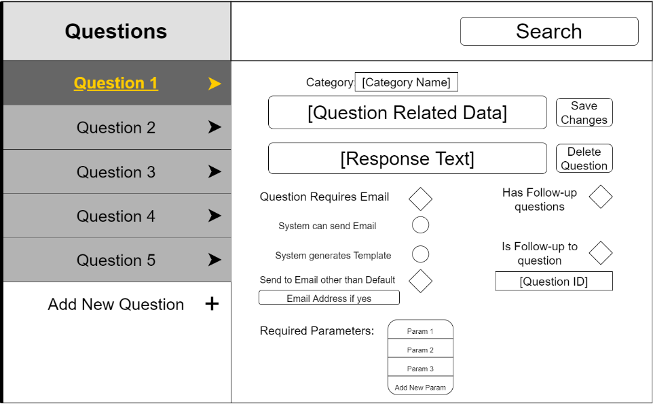
\includegraphics[width=0.75\linewidth]{images/original-questions-panel.png}
    \caption{The original questions panel.}
\end{figure}



 


\subsection{Original Ideas}

\subsubsection{Maya Awad}

\begin{enumerate}
    \item As far as I can tell from research, we will probably end up using Python.
    \begin{itemize}
        \item Update: This does not seem to have changed, though we may have to lean on JavaScript for the front end a little.
    \end{itemize}
    \item I think we could use TensorFlow for the machine learning process.
    \item A special case for Foundation Exam questions would be neat.
    \item A student front-end (the actual chatbot) vs. faculty front-end that allows for new questions and answers to be added/deleted.
    \item Building off of the “faculty front-end,” do we need a system that auto-trains the bot on the new word or would just feeding it a bunch of examples be enough for the existing system to work off of?
    \item Would the faculty front end be an entirely separate project? It probably doesn’t have to look nearly as nice as the front-end everyone will see.
    \begin{itemize}
        \item Update: To be deliberated farther but it is becoming more likely that the faculty front end will come with this project.
    \end{itemize}
    \item What will the front-end be written in? Will we have to brave the wastelands of JavaScript? I assume we could keep the interface super simple so it may not matter in the end.
    \begin{itemize}
        \item As stated before, we will likely use at least a little bit of JavaScript
    \end{itemize}
    \item Stretch Goal: Access from the UCF mobile app? I imagine it would only have to be the front end that would have to get made from scratch, then it could just make calls to wherever the chatbot is being hosted. 
    \begin{itemize}
        \item Update: To be deliberated on farther, it is likely not necessary however.
    \end{itemize}
    \item Would the chatbot have its “own” email? Would the chatbot be able to email on behalf of the student? I think that if the student must send an email, they should do it themselves so that the advisor can get back to them directly. The chatbot should provide which information should be included by the student, but the rest is up to them.
    \begin{itemize}
        \item Still under deliberation, however the problem of the advisor being unable to reply directly to the student by hitting “reply” is a large downside. 
    \end{itemize}
    \item We would likely want a “this link is broken” option when the bot provides a link to a form or something, since in my experience a lot of links on the UCF website are broken.
    \item I still want it to be related to the mascot by calling the chatbot Knightroid (Knightro + Android). I would love to incorporate the Pegasus as well, but I haven’t thought of a way to do so yet. Maybe while the chatbot is working it’s the little loading symbol.
    \item In the event that two different answers get the same percent likelihood to be a relevant answer, how do we resolve the tie? Do we show both answers and let the student pick? Do we program in follow up questions?
    \item Will this chatbot be visible to everyone or just registered students? I think I would like it to just be on the CS/IT website as opposed to somewhere like WebCourses, since I believe it would be more helpful to people who haven’t even enrolled yet, though this may involve fielding an even wider array of questions.
    \begin{itemize}
        \item It has been deliberated on and will likely be deliberated on farther. On one hand a very common email starts with “I just started here/got accepted” and it may be that the student does not have a login yet. On the other hand, no level of login increases the potential amount of load on the app and would potentially cost more money should we use a paid app, and this in turn would be susceptible to trolling that has a real-world monetary impact.
    \end{itemize}
    \item In the event that a question has no match above 50\%, the chatbot may ask the user to rephrase, and after 3 attempts it will just shoo them off to a human. I would like this if we can to give suggestions to the user on what should be in the email they will hopefully send. This could be things like “please include your UCF ID and your major”.
    \item What to do when it isn’t a question. Should it treat it as a question regardless? Should it give a “could you please rephrase that?” I believe the second option would be easier to implement since it would kind of already be there, otherwise we would have to program more, extra responses for non-questions. 
    \item Sentiment analysis. While I was researching NLP, one of the projects that came up was sentiment analysis. Should we be able to tell that the user is, say, obviously typing in frustration or just yelling obscenities.
    \item Ticket/Chat Logs. Should we even keep a log of what was said and for how long? I can’t think of a good reason why someone would want to look back at exactly what was said aside for testing reasons. Additionally, quite a few chatbot interactions will simply be pointing someone in the right direction and they wouldn’t necessarily need to input any identifying information, rendering a ticket log basically useless. 
    \begin{itemize}
        \item This question has been kicked back and forth quite a lot, and the answer has changed more than once. At first it was a possible breach of privacy to record everything someone typed, but then it “would be useful”.
    \end{itemize}
    \item Statistics. I think it would be cool if we kept statistics on the most accessed questions/answers in the database, it could show where information is lacking and not reaching students as effectively as it could.
    \begin{itemize}
        \item This could be another table in the database, or another column, or both. Would need to look into some sort of scheduled routine that keeps track of how often something got asked in the past month and find the most frequently asked questions of the last month and have them be suggestions for the beginning of a conversation with the chatbot.
    \end{itemize}
    \item Grab dates off of the UCF calendar page and be able to tell the user, for example, when the withdrawal deadline is.
    \begin{itemize}
        \item Possible to scrape data from a site but what if the format changes?
    \end{itemize}
    \item Rating “how helpful was this” system? Similar to statistics but users could leave comments.
\end{enumerate}

In Assignment 3, we each created a list of 20 ideas (as seen above) that we presented to each other, reflecting back, some of these ideas can already be struck out. Many of these are ideas that rely on training a chatbot from scratch, which we have decided not to do based on professor feedback i.e. “don’t reinvent the wheel”.  2, 5, 12, 15, 16 are all ideas that are to be entirely scrapped due to this development. This includes using TensorFlow, having a separate AI for the faculty front end, the event of a tie, non-question questions, sentiment analysis. 

There are also ideas that have been deliberated on more since and do not have definitive answers. 1, 6, 8, 9, 13, 17, 18, and 19 are ideas that require further investigation, some of which in this will be handled in this section.

\subsubsection{Owen Brahms}

\begin{enumerate}
    \item Split questions into broad Topics and more specific Questions, to allow the system to be a bit more modular.
    \item Each question sends a “Ticket” to the system backend. If that “Ticket” matches existing tickets, it receives the same answer. Otherwise, the system will analyze the ticket to determine the best person it should be sent to.
    \item System uses machine learning to analyze both emails sent by advisors and emails sent by students to determine the best possible responses to a given question.
    \item System uses machine learning on student questions to determine the most common formats of questions and how they should be split to receive their associated answers.
    \item Randomly answer questions from a pool of potential answers.
    \item Begin by asking if the student has any questions and let the student make the first move. Then, analyze the question asked to determine what the most accurate “Topic” is and the most accurate sub-question. Then, confirm with the student that was the question they asked.
    \item Begin by prompting the user with the possible Topics, then with the possible sub-questions, and ask the user to pick from the available options.
    \item Just make an FAQ with a backend to update the questions and answers.
    \item Have a list of potential questions, but allow students to ask questions outside of that list. If the question is similar enough to another question, that answer will be given and the student will be asked if that solved their problem. If not, the student will be prompted to send an email to the person most appropriate to answer their question.
    \item Make a mobile app or integrate system with UCF app for easy access.
    \item Integrate system into Student Center so it can tailor its answers to the specific students’ information.
    \item In the back-end, allow advisors to upload a copy of a specific document which should accompany a specific answer, which can be sent to a student if it is necessary for the request they are making.
    \item Allow advisors to upload a copy of a document to give to a student, but only provide it to the student after asking if they’d like a copy of the document and they respond in the affirmative.
    \item Begin by asking the student for their Major and using that as a basis for the initial “Topic”.
    \item Begin by asking the student for their Major but also give a list of potential majors they can select which the system is capable of managing. If the user selects a major not on the list, the system will direct them towards the appropriate department.
    \item When a question does not have an answer and must be sent to an advisor, add that question to the backend and request that an advisor fill in the answer.
    \item Set up a ticketing system which can handle both the questions and the responses. If a question has a set response, that response will automatically be sent. If it does not, the appropriate advisor will be alerted to answer said question. They will then be given the option to decide if that answer should be used for any similar questions.
    \item In addition to the above idea, advisors can also mark questions as always needing an advisor response.Responses to those questions will not be given additional options.
    \item The system can automatically send emails to the necessary people for the specified question, given that the advisor who input the appropriate answer also gave an email address for the question to go to. There would also be fields for “required information” for any such follow-up question.
    \item Multi-part questions. For example, asking for an override for a class, the system will ask if you already have your override form filled out. If yes, it will prompt you to send an email. If no, it will provide you with the form and explain how it should be filled out for the question you’ve asked.
\end{enumerate}

\subsubsection{Reagan Chapman}

\begin{enumerate}
    \item The bot could ask for each student’s UCF ID/Name/Major at the beginning of the conversation. 
    \item The bot could request personal information only when required to complete a task (this is in conflict with number 1). 
    \item If giving the bot personal information is optional, we can incentivize it when it is beneficial. For example, “If you give me your UCF ID, I can let your adviser know that I was unable to solve your problem, which will make this a high priority question for them.” 
    \item The bot could ask at the end if the conversation solved the student’s issue. 
    \item If we decide to have the bots send emails to advisers, we should give the students the opportunity to modify the content of the message, where they see fit. 
    \item The bot could provide information in an email that will help the appropriate person resolve the issue as efficiently as possible. For example, if the fulfillment of a request requires confirmation that the student has things like the appropriate GPA, prerequisites met, written approval, etc., these things should be asked of the student in the conversation with the chat bot, before the email is sent. Then, the email can show the recipient that all of those things are met, saving an additional pair of emails. 
    \item The bot could be named the “Myah” (Make Your Advisor Happy) Bot.  
    \item There could be spellcheck in the typing interface so that there will be less of a chance that students will type a word that the bot will not understand. If what is typed will be viewed as nonsensical to the bot, it could be underlined with the traditional, red squiggly. 
    \item If the question that the student asks seems to be off-topic, the bot could ask the student to confirm what they are saying. For example, “Is your question about Bright Futures?”, just to ensure that they are not dismissing a legitimate question by accident. 
    \item If the question is off-topic, but the relevant information is still easily available, the bot can direct them to it. For example, in line with number 9, if the student answered, “Yes”, a response could be, “Unfortunately, that is outside of my area of expertise, but information about scholarship eligibility can be found here \_\_\_\_\_, or you can contact \_\_\_\_\_.” 
    \item If, as the professor said, it is hard to get the bot to understand what is being asked, we can rely on a series of questions like places such as banks use when you call them on the phone. “If your call is about \_\_\_\_, press 1”. Instead of pressing one, we could just give them a series of topics and have them type in the topic that they want to discuss. We could also just say, “Type in a few words about the topic of your issue.” 
    \item I think that swearing and “abusive language” should just be ignored. I do not think it really matters if our bot’s feelings are hurt. Definitely not worth getting the student in trouble. They could just be playing around. 
    \item In the back end, it would be helpful if advisers could add or modify questions that they expect to be asked. 
    \item The questions added by advisers could be parsed for essential language. For example, “Will next semester be online due to coronavirus, or will it be in person/face-to-face?” The only essential keywords may be something like “next semester online/in person/face-to-face coronavirus”.  
    \item Each real question could then be compared to all the parsed keywords. This could be done by rating how closely that the real question and the keywords match. The best match could then be addressed by saying, “So, you would like to know about updates about our return to campus?” If the student says, “yes”, the bot could give them a link to the updates. 
    \item We could have a metric that tells the advisers what questions are asked most often. 
    \item We could have a metric that tells the advisers what questions receive answers that students are satisfied with and which ones do not. 
    \item We could test Dr. Heinrich’s inbox, containing previous emails, in order to come up with metrics of email reduction. 
    \item Metrics could include how many emails should have never been sent to the adviser in the first place. 
    \item Metrics could include how many emails that fall into the adviser’s expertise, but can easily be solved by the bot.
\end{enumerate}

\subsubsection{Raj Patel}

\begin{enumerate}
    \item Starting from the lowest tier have a login system “depending on the requirements” then maybe have a frequently asked questions pane or questions suggestion introduction as user visits the bot at the first glance after logging in, to get an idea of what’s something the bot can answer or help with.
    \item Use a rule-based approach and mix it up with some NLP and start from a broader list of questions and streamline them as the users responds depending upon the keywords or the predetermined word cloud from previous conversations/emails.
    \item Use technologies and machine learning platforms such as TensorFlow to train existing models or create new ones as time progresses for more customization and adding new information for processing.
    \item As far as the view goes we can possibly have an active assistant on the advising page for the department at all times and the student can click on it to open up the chatbot and get assistance regarding many potential issues or queries that can be solved without emailing the advisor or email them after running through the bot which potentially will be assisted by the bot.
    \item For the names I don’t have any specifics but maybe knightron (like Ultron) or something that we all discussed in our past meeting was KnugVising (relating to nugget). 
    \item Collect information from the student right at the beginning such as UCF Id and name to start with and then guide them through by asking relevant question to reach the finish line.
    \item If the bot isn’t able to answer the question but it can detect that the question pertains to the advisor the bot can generate a pre written email in the format that the advisor desires to make it very easy for the advisor to decode and look for what they need from user in their desired format.
    \item Users get the chance to edit or tweak that pre-written email if they want to add any additional comments or questions, or it can also generate a template structured by the advisor for the specific issue (such as override form or transfer process) that the student could fill out so there is less back and forth email conversations to save time for both parties.
    \item Add a filter to detect keywords that don’t pertain to the specific department and re-route the student to the department that is responsible such as financial aid and the bot can ask a question such as do you need assistance with financial aid? If the student says ‘yes’ then the bot responds with the department email and a way to contact them and reboot the process to ask again if there’s anything else that needs any assistance.
    \item The bot is constantly improving and learning from the type of questions as an added functionality to improve efficiency in terms of time and results this can be done through some machine learning techniques and from what I’ve been reading it seems python is an ideal language to handle such a project.
    \item Design the web-app’s backend in a way that the advisor can get privileges to tweak the model or add words to the cloud or add question types as time progresses. One such situation could be COVID related questions that would not be stored in the bot system so the advisors can go and tweak such things.
    \item When a new circumstance or question is asked, assign a flag and add it to the list of unusual questions and have the advisor is able to review. If that question is valid and relates to their department then the advisor can input that question and the answer to it to the database.
    \item In terms of growth a model for each department with different answers for different question each for different departments can be made in the future and used as another senior design project in the coming time. It can certainly be set up to make it easier to expand to other departments.
    \item Implement a privilege system with and admin privilege, a moderator privilege, and a common student view functionality. Admin can be the UCF IT department and moderators could be the advisors. Admins can edit departments and moderators can add or delete new questions relating to their departments, but this is more on the side of setting up the infrastructure for future long-term goals.
    \item Potentially bring this project to a mobile and tablet platform for ease of use and increasing accessibility at the same time.
    \item The bot could be capable of suggesting the right form for the right question for the student to fill out and make sure the margin of error can be minimized.
    \item Bot theme could be the mascot hanging in the corner of the page with an auto hide and show feature.
    \item A data sorting system for the advisor sort of like a plugin for the advisors’ email to sort the email regarding the flag sent via the bot (included in the prewritten email) to further ease the work of the advisor. This could have some legal issues, but more research needs to be done regarding this idea.
    \item Keep the possibility to release updates in the future so make it with a long-term vision and use the most updated technologies to make it a lot easier and maintainable, while providing essential features and solutions.
    \item Add a speak feature to speak to the bot (Alexa/Siri/google etc.) or just a plain simple mic that can convert words to text.
\end{enumerate}

\subsubsection{Carlos Santiago Bañón}

\begin{enumerate}
    \item We could use either the IBM Watson, Amazon Lex, Azure Bot Service, Google DialogFlow, or any other main chatbot platform.
    \item We could develop our system using Python, which has excellent support for Natural Language Processing libraries.
    \item We could have it all set up in an independent web application to ensure the highest quality possible, much like the mySchedule Builder and Pegasus Path tools.
    \item The chatbot could be part of the existing CECS website for ease of access, possibly having to work with older technologies.
    \item We could have a special portal for advisors to access back-end information.
    \item We could have a cool mascot represent the chatbot for a high-quality interaction with the user. Examples could be Knightro, Knugget, Citronaut, or any new custom mascot.
    \item We should mine a large dataset to have a central set of training and testing examples to train our chatbot.
    \item Our chatbot should have a built-in detector for abuse and profanity.
    \item The system could have a ticketing system that reports back to advisors to track relevant interactions.
    \item The system could provide a choice of answers to the user for better communication.
    \item The system could be triggered by voice in addition to text.
    \item We need to establish important evaluation metrics for our system (e.g., accuracy, F1 score, precision, recall, etc.)
    \item The system could use new requests for self-improvement.
    \item The system should send the user an email with a summary of the interaction for their records.
    \item There needs to be some marketing campaign once the system is completed to let students know of its existence.
    \item The system should have a “Did you mean \_\_\_?” option in case it does not understand a particular request.
    \item The system could recommend courses to students based on their academic history and interests. This could answer the “which courses should I take next?” line of questions.
    \item The system should have a directory of important UCF contact information.
    \item The system should respond with empathetic messages to ensure trust is established.
    \item When in doubt, the system should always point to an academic advisor.
\end{enumerate}











\pagebreak
\section{Budgeting and Financing}

In the early stages of our system design, some key research was done in the area of budgeting and financing. However, after consulting our sponsor and many team discussions, our budget was determined to be nonexistent.

While looking at existing chatbot platforms, our research produced Table (???), containing pricing information for the top contenders. These were Google DialogFlow, Amazon Lex, IBM Watson, Microsoft’s Azure Bot Service, and Wit. However, as described in section (???), we eventually decided to pursue the idea of implementing our own system from scratch using deep learning libraries (e.g., PyTorch, TensorFlow, Keras, etc.) to gain a higher level of customization. Therefore, the product is expected to not be of any cost to the university.

\begin{center}
\begin{table}[h]
\centering
    \begin{tabular}{ L{2cm} L{3cm} L{4.5cm} }
    
        \toprule
        \textbf{Platform} & \textbf{Languages} & \textbf{Pricing} \\

        \midrule
        Google Dialogflow & 20+ & Standard Plan: Free, Enterprise: 0.002 Per Request \\

        \midrule 
        Amazon Lex & Only U.S. English & Voice: \$0.004 Per Request, Text: \$0.00075 Per Request \\

        \midrule
        IBM Watson & 10+ (Beta) & Free Plan: 10k Messages Per Month, Paid Plans: Starting at \$0.0025 Per Message \\

        \midrule
        Microsoft’s Azure Bot Service & 5+ & Free Plan: 10k Messages Per Month, Paid Plans: \$0.5 Per 1,000 Messages (Plus Azure Service Costs) \\

        \midrule
        Wit & 50+ & Free for personal and commercial use. \\

        \bottomrule
        
    \end{tabular}
    \caption{Chatbot platform pricing.}
\end{table}
\end{center}

\pagebreak
\section{Project Management}

\subsection{Product Backlog}

The backlog used to manage the development of this product can be found in Table (???).

\begin{center}

        \begin{longtable}{ L{1.5cm} L{4cm} L{1.5cm} L{3cm} L{1.5cm} }
        \caption{Product backlog.} \\
        \toprule
        \textbf{Code} & \textbf{User Story} & \textbf{Priority} & \textbf{Component} & \textbf{Points} \\
        \toprule
        \endhead
        DAT-02 & As an administrator, I can add recognized questions to any department.                                                            & High   & Database, Faculty   & 0           \\
        \midrule
        DAT-03 & As an administrator, I can add responses to recognized questions in any department.                                               & High   & Database, Faculty   & 0           \\
        \midrule
        DAT-05 & As an administrator, I can delete recognized questions from any department.                                                       & High   & Database, Faculty    & 0          \\
        \midrule
        DAT-06 & As an administrator, I can delete responses to recognized questions from any department.                                          & High   & Database, Faculty    & 0          \\
        \midrule
        DAT-08 & As an administrator, I can edit recognized questions from any department.                                                         & High   & Database, Faculty    & 0          \\
        \midrule
        DAT-09 & As an administrator, I can edit responses to questions from any department.                                                       & High   & Database, Faculty    & 0        \\
        \midrule
        DAT-10 & As an administrator, I can see all data metrics.                                                                                  & High   & Database, Faculty    & 0           \\
        \midrule
        DAT-11 & As an administrator, I can see all recognized questions and responses.                                                            & High   & Database, Faculty    & 0         \\
        \midrule
        DAT-12 & As an administrator, I can see the most frequently-asked questions in any department.                                             & High   & Database, Faculty    & 0           \\
        \midrule
        DAT-14 & As an advisor, I can add recognized questions to my department.                                                                   & High   & Database, Faculty    & 0             \\
        \midrule
        DAT-15 & As an advisor, I can add responses to recognized questions in my department.                                                      & High   & Database, Faculty    & 0          \\
        \midrule
        DAT-17 & As an advisor, I can delete recognized questions from my department.                                                              & High   & Database, Faculty    & 0         \\
        \midrule
        DAT-20 & As an advisor, I can edit recognized questions in my department.                                                                  & High   & Database, Faculty    & 0         \\
        \midrule
        DAT-21 & As an advisor, I can edit responses to recognized questions in my department.                                                     & High   & Database, Faculty    & 0         \\
        \midrule
        DAT-22 & As an advisor, I can see my department's data metrics.                                                                            & High   & Database, Faculty    & 0         \\
        \midrule
        DAT-23 & As an advisor, I can see the most frequently-asked questions in my department.                                                    & High   & Database, Faculty    & 0          \\
        \midrule
        DOC-01 & As a sponsor, I am provided with a thorough system design document.                                                               & High   & Documentation       & 0 \\
        \midrule
        DOC-02 & As an administrator, I am provided with thorough documentation to know how to use the faculty system.                             & High   & Documentation       & 0\\
        \midrule
        DOC-03 & As an advisor, I am provided with thorough documentation to know how to use the faculty system.                                   & High   & Documentation       & 0   \\
        \midrule
        DOC-04 & As a sponsor, I am provided with a name for the product.                                                                          & High   & Documentation       & 0  \\
        \midrule
        FNC-01 & As a student, I can ask a question to the chatbot.                                                                                & High   & AI, Student          & 0    \\
        \midrule
        FNC-02 & As a student, I can get a response from the chatbot.                                                                              & High   & AI, Student          & 0   \\
        \midrule
        FNC-03 & As a student, I can get an accurate response from the chatbot.                                                                    & High   & AI, Database, Student & 0   \\
        \midrule
        FNC-04 & As a student, I can see examples of questions I can ask the chatbot.                                                              & High   & Student             & 0    \\
        \midrule
        FNC-05 & As a student, if the chatbot does not know answer to a question, I can be directed to someone who does.                           & High   & AI, Database, Student & 0    \\
        \midrule
        FNC-06 & As a student, if the chatbot sends an email on my behalf, I can set a custom reply-to email.                                      & High   & Student             & 0    \\
        \midrule
        FNC-07 & As a student, if the chatbot suggests sending an email to my advisor (with attachments), I can see a template of what to include. & High   & AI, Database, Student & 0    \\
        \midrule
        FNC-08 & As a student, if the chatbot suggests sending an email to my advisor (without attachments), it can send the email for me.         & High   & AI, Database, Student & 0    \\
        \midrule
        FNC-09 & As an advisor, if the chatbot sends me an email, I can see a transcript of the conversation with the student.                     & High   & Faculty, Student     & 0    \\
        \midrule
        FNC-13 & As a student, I can see the most frequently-asked questions.                                                                      & High   & Database, Student    & 0      \\
        \midrule
        FNC-14 & As a student, if the chatbot does not understand my question after a number of times, I can be redirected to my advisor.          & High   & AI, Database, Student & 0      \\
        \midrule
        FNC-15 & As a student, if the chatbot does not understand my question, I have the chance to clarify myself.                                & High   & AI, Database, Student & 0  \\
        \midrule
        INT-01 & As a student, I can access the chatbot.                                                                                           & High   & Student             & 0     \\
        \midrule
        INT-02 & As a student, I can ask a question to the chatbot using my voice.                                                                 & High   & Student             & 0      \\
        \midrule
        SEC-01 & As a student, I can log in to the system using my UCF authentication credentials.                                                 & High   & Student             & Security       \\
        \midrule
        SEC-02 & As a student, I can only use my UCF Knights email for communicating with my advisor.                                              & High   & Student             & 0  \\
        \midrule
        SEC-03 & As an advisor, I can log in to the system using my UCF authentication credentials.                                                & High   & Faculty             & 0     \\
        \midrule
        DAT-24 & As an administrator, I can add advisor accounts to the faculty system.                                                            & Medium & Database, Faculty    & 0          \\
        \midrule
        DAT-25 & As an administrator, I can add departments to the faculty system.                                                                 & Medium & Database, Faculty    & 0             \\
        \midrule
        DAT-26 & As an administrator, I can delete advisor accounts from the faculty system.                                                       & Medium & Database, Faculty    & 0              \\
        \midrule
        DAT-27 & As an administrator, I can delete departments from the faculty system.                                                            & Medium & Database, Faculty    & 0              \\
        \midrule
        DAT-28 & As an administrator, I can edit advisor accounts in the faculty system.                                                           & Medium & Database, Faculty    & 0              \\
        \midrule
        DAT-29 & As an administrator, I can edit departments in the faculty system.                                                                & Medium & Database, Faculty    & 0            \\
        \midrule
        DAT-30 & As an administrator, I can see all advisor accounts in the faculty system.                                                        & Medium & Database, Faculty    & 0              \\
        \midrule
        DAT-31 & As an administrator, I can see all departments in the faculty system.                                                             & Medium & Database, Faculty    & 0          \\
        \midrule
        DAT-32 & As an administrator, I can see all user feedback.                                                                                 & Medium & Database, Faculty    & 0         \\
        \midrule
        DAT-33 & As an advisor, I can see my department's user feedback.                                                                           & Medium & Database, Faculty    & 0       \\
        \midrule
        FNC-10 & As a student, I am notified if the chatbot sends any information on my behalf to an advisor.                                      & Medium & Student             & 0     \\
        \midrule
        FNC-11 & As a student, I am provided with the option to receive a transcript email after my conversation with the chatbot.                 & Medium & Student             & 0    \\
        \midrule
        FNC-12 & As a student, I can provide anonymous user feedback.                                                                              & Medium & Database, Student    & 0     \\
        \midrule
        FNC-16 & As a student, if the chatbot suggests sending an email, I have the option to decline.                                             & Medium & AI, Student          & 0       \\
        \midrule
        INT-03 & As a student, I can access the chatbot from all main browsers.                                                                    & Medium & Student             & 0        \\
        \midrule
        SEC-04 & As an administrator, I can edit account permissions in the faculty system.                                                        & Medium & Database, Faculty    & 0         \\
        \midrule
        DAT-01 & As an administrator, I can add forms to any department.                                                                           & Low    & Database, Faculty    & 0            \\
        \midrule
        DAT-04 & As an administrator, I can delete forms from any department.                                                                      & Low    & Database, Faculty    & 0         \\
        \midrule
        DAT-07 & As an administrator, I can edit forms in any department.                                                                          & Low    & Database, Faculty    & 0            \\
        \midrule
        DAT-13 & As an advisor, I can add forms to my department.                                                                                  & Low    & Database, Faculty    & 0           \\
        \midrule
        DAT-16 & As an advisor, I can delete forms from my department.                                                                             & Low    & Database, Faculty    & 0           \\
        \midrule
        DAT-18 & As an advisor, I can delete responses to recognized questions in my department.                                                   & Low    & Database, Faculty    & 0         \\
        \midrule
        DAT-19 & As an advisor, I can edit forms in my department.                                                                                 & Low    & Database, Faculty    & 0               \\
        \midrule
        DOC-05 & As a sponsor, I am provided with consistent branding for the product.                                                             & Low    & Documentation       & 0  \\
        \bottomrule \\

        \end{longtable}

\end{center}



























































\end{document}
